\chapter{Schwingungen und Wellen}
\label{kap_schwingungen-und-wellen}




\section{Freie Schwingung}
\label{kap_freie-schwingung}

\begin{Def}
   [Freie Schwingung]\index{freie Schwingung} Bei einer \textbf{freien
     Schwingung} treten keine externen Kr"afte auf.
\end{Def}

Die hier auftretenden Kr"afte sind stets
\begin{itemize}
\item Die tr"age Kraft $F_T = m \ddot x$
\item eine \emph{lineare} R"uckstellkraft.
\end{itemize}
Je nach \emph{Art} des Pendels (vgl. Abb. \ref{abb_pendel}) unterscheiden sich die R"uckstellkr"afte:
\begin{description}[\setlabelstyle{\bfseries\slshape}]
\item[\index{Federpendel}Federpendel] Federkraft\footnote{Das "`$-$"'
     kommt daher, dass wenn die Auslenkung $x$ (oBdA) in die positive
     Richtung geht, die Federkraft in die \emph{Gegenrichtung} -- also
     in die negative Richtung -- zeigt.}: $F_R = - D \cdot x$
\item[\index{Torsionspendel}Torsionspendel] Federkraft\footnote{mit
     der \emph{Federrichtgr"o"se} $D^*$, mit $D^* :=
     \frac{F}{\varphi}$} $F_R = -D^* \cdot \varphi$ (hier ist $F_T = I
   \ddot \varphi$)
\item[\index{Fadenpendel}Fadenpendel] $F_R = -F_G \cdot \sin \varphi =
   -mg \cdot \sin \varphi \approx -mg \cdot \varphi$
\end{description}

Da hier keine externen Kr"afte angreifen, muss sich die Tr"age Kraft
$F_T$ komplett aus der R"uckstellkraft ergeben\footnote{Dass die Tr"age
  kraft vorhanden sein muss, ergibt sich daraus, dass ein Pendel
  st"andig seine Geschwindigkeit "andert. So muss st"andig eine
  Beschleunigung wirken und mit $F = ma$ muss damit st"andig eine Kraft
  wirken.} -- schlie"slich ist keine andere Kraft da:
\begin{equation}
   \label{eq:101}
   F_T = F_R
\end{equation}
Am Beispiel des Federpendels gilt dann:
\begin{equation}
   \label{eqn_freie-schwingung}
   m\ddot x = - D x ~ \Leftrightarrow ~ \boxed{m\ddot x + Dx = 0}
\end{equation}
Dies ist die verallgemeinerte \textbf{Bewegungsgleichung} einer freien
Schwingung!

Hier haben wir stets eine \emph{Differentialgleichung} zu l"osen -- wir
haben $x(t)$ zu bestimmen. Hier hilft der Ansatz
\begin{equation}
   \label{eq:103}
   x(t) = \hat x \cdot \sin(\omega t + \varphi_0)
\end{equation}
\begin{Def}
   \label{def_harmonische-schwingung} Wir bezeichnen eine Schwingung
   als \textbf{\index{harmonische Schwingung}harmonische Schwingung}, wenn der Systemparameter (die
   Koordinate) einer \emph{Sinusfunktion} in der Zeit folgen kann.
\end{Def}
Durch Ableiten und Einsetzen erh"alt man hierbei mit \eqref{eqn_freie-schwingung}:
\begin{equation}
   \label{eq:104}
   \omega = \sqrt{\frac{D}{m}}
\end{equation}
und damit eine Schwingfrequenz von 
\begin{equation}
   \label{eq:105}
   \nu = \frac{1}{T} =  \frac{\omega}{2\pi} = \frac{\sqrt{D}}{2\pi \sqrt{m}} 
\end{equation}
Die Gleichungen f"ur die anderen Schwingungen lassen sich analog l"osen.


\begin{figure}
   \centering
   \subfigure[Torsionspendel]{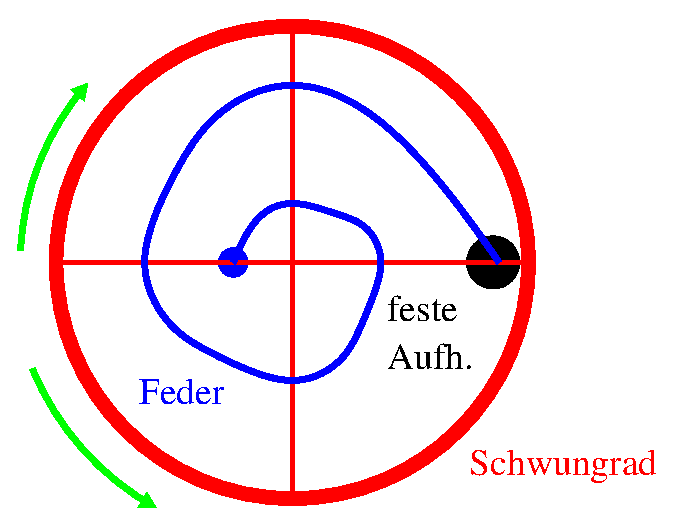
\includegraphics[width=0.3\textwidth]{bilder/torsionspendel}}
   \subfigure[Federpendel]{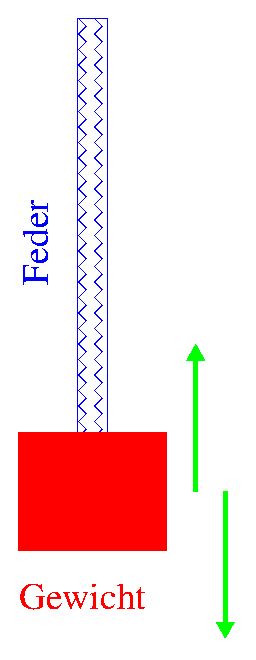
\includegraphics[height=0.22\textheight]{bilder/federpendel}} 
   \subfigure[Fadenpendel]{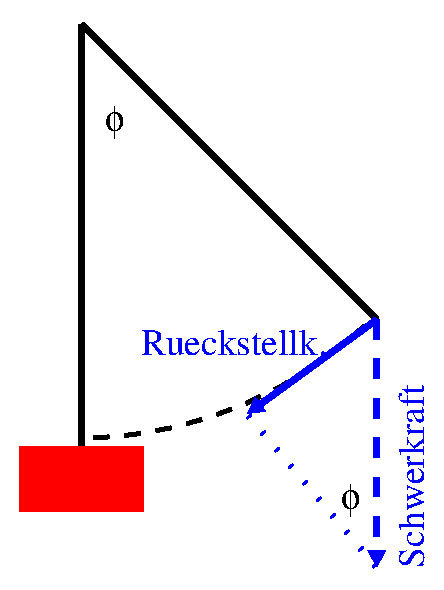
\includegraphics[width=0.3\textwidth]{bilder/fadenpendel}}
   \caption{Verschiedene Sorten von Pendeln}
   \label{abb_pendel}
\end{figure}








\section{D"ampfung}
\label{kap_dampfung}

Nun k"onnen neben der R"uckstellkraft und der Tr"agen Kraft noch
weitere Kr"afte angreifen, die wir meistens vernachl"assigen;
bspw. \textbf{\index{Reibung}Reibungskr"afte}. Die Reibung
("`\index{D"ampfung"'}D"ampfung"') ist meistens von der
Geschwindigkeit abh"angig:
\begin{equation}
   \label{eq:102}
   F_D = - \gamma \dot x
\end{equation}

Wir erhalten dann die \textbf{Bewegungsgleichung} wieder, weil sich
die Tr"age Kraft als Summe der andere Kr"afte darstellen l"asst:
\begin{equation}
   \label{eqn_schwingung-reibung}
   F_T = F_R + F_D ~ \Leftrightarrow ~\boxed{ m\ddot x + \gamma \dot x
     + Dx = 0 }
\end{equation}
Wir sprechen dann von einer \textbf{freien ged"ampften Schwingung.}

Diese freie Schwingung ist keine \emph{harmonische Schwingung} mehr!



\subsection{Geratener Ansatz}
\label{kap_geratener-ansatz}



Als Ansatz zum L"osen der
DGL\footnote{\textbf{D}ifferenzial\textbf{gl}eichung} verwenden
(raten)\footnote{Diese Technik wird auch als "`\emph{clever guess}"'
  bezeichnet.} wir
\begin{equation}
   \label{eq:106}
   \boxed{x(t) = \hat x \cdot \exp(-\delta t) \cdot \sin(\omega t + \varphi_0)}
\end{equation}
Durch zweimaliges Ableiten erhalten wir
\begin{equation}
   \label{eq:108}
   \dot x = - \delta \cdot x + \hat x \cdot \omega \cdot \exp(-\delta t) \cdot \cos(\omega t + \varphi_0)
\end{equation}
und 
\begin{equation}
   \label{eq:110}
   \ddot x = (\delta^2 - \omega^2 )\cdot x - 2 \cdot \hat x \cdot \delta \omega \cdot
   \exp(-\delta t) \cdot \cos(\omega t + \varphi_0) 
\end{equation}
und durch Einsetzen in \eqref{eqn_schwingung-reibung} (mit der
Vereinfachung $\theta := \omega t + \varphi_0$):
% \footnote{Dabei
%   steht $\sin$ f"ur $\sin(\omega t + \varphi_0$ und $\cos$
%   entsprechend... $\sin$ ist also hier in gewissem Sinne eine einfache
%   Variable anstatt einer Funktion. }
\begin{equation}
   \label{eq:109}
%    \hat x \exp(-\delta t) 
% \left [
% \delta^2 m - \omega^2 m - 2 \delta \omega m\cos(\omega t +
% \varphi_0) 
% -
% \delta \gamma  \sin(\omega t + \varphi_0) + \omega \gamma 
% \cos(\omega t + \varphi_0)
% +
% D \sin(\omega t + \varphi_0)
%  \right ] = 0
   \hat x \exp(-\delta t) 
\left [
\delta^2 m \sin\theta - \omega^2 m \sin\theta - 2 \delta \omega m\cos\theta
-
\delta \gamma  \sin\theta + \omega \gamma 
\cos\theta
+
D \sin\theta
 \right ] = 0
\end{equation}
Da $\hat x \exp(-\delta t) \neq 0$ ist, k"onnen wir den Teil in eckigen
Klammern umfornem:
\begin{equation}
   \label{eq:111}
 [ \delta^2m - \omega^2m - \delta \gamma + D ] \sin\theta + [-2\delta\omega m +
 \omega \gamma] \cos\theta = 0
\end{equation}
Da Sinus und Cosinus beide Null werden k"onnen, aber nicht
\emph{gleichzeitig} -- die Gleichungen aber für jede Zeit $t$ und
damit jede Phase $\theta$ -- , muss jeder der Terme in eckigen
Klammern verschwinden, weil wenn $\cos\theta = 0$ gilt, verschwindet
der rechte Term und dann muss der linke ebenfalls verschwinden. Weil
an dieser Stelle $\sin\theta \neq 0$ ist, muss nach dem \emph{Satz vom
  Nullprodukt} die Klammer verschwinden; wir erhalten also
\begin{eqnarray}
   \label{eq:112}
    \delta^2m - \omega^2m - \delta \gamma + D  &=& 0\\
\label{eq:113}
-2\delta\omega m +
 \omega \gamma &=& 0
\end{eqnarray}
Aus \eqref{eq:113} gilt 
\begin{equation}
   \label{eq:114}
   \delta = \frac{\gamma}{2m}
\end{equation}
und damit und mit \eqref{eq:112} gilt
\begin{equation}
   \label{eq:115}
\omega^2 =  \frac{D}{m} - \frac{\gamma^2}{4m^2}
\end{equation}
Aus Kap. \ref{kap_freie-schwingung}  wissen wir,
die Frequenz der zugeh"origen \emph{freien Schwingung}:
\eqref{eq:104}. Diese nennen wir hier $\omega_0$. Mit \eqref{eq:114}
gilt also:
\begin{equation}
   \label{eq:116}
\boxed{   \omega = \sqrt{\omega_0^2  -  \delta^2}  }
\end{equation}




\subsection{Allgemeiner Ansatz}
\label{kap_allgemeiner-ansatz}

Der Allgemeine Ansatz zur L"osung einer DGL wie
\eqref{eqn_schwingung-reibung} ist 
\begin{equation}
   \label{eq:119}
  x =    x(t) = c \exp(\lambda t)
\end{equation}
Durch Ableiten 
\begin{eqnarray}
   \label{eq:120}
   \dot x &=& \lambda \cdot x\\
 \ddot x &=& \lambda^2 \cdot x
\end{eqnarray}
und Einsetzen
\begin{equation}
   \label{eq:121}
   m \lambda^2 x + \gamma \lambda x + D x = 0
\end{equation}
kommt man (durch K"urzen mit $x$ da $x \neq 0$ f"ur $c \neq 0$) auf das
\emph{\index{characteristisches Polynom}characteristische Polynom}
\begin{equation}
   \label{eq:122}
    m \lambda^2 + \gamma \lambda + D  = 0
\end{equation}
welches wir mit der Mitternachsformel l"osen k"onnen:
\begin{equation}
   \label{eq:123}
   \lambda = \frac{-\gamma \pm \sqrt{\gamma^2 - 4Dm}}{2m}
 = 
\frac{- \gamma }{2m} \pm \sqrt{\frac{\gamma^2}{4m^2} - \omega_0^2}
=:
- \delta \pm \underbrace{\sqrt{\delta^2 - \omega_0^2}}_{\I \omega}
\end{equation}
Die Allgemeine L"osung f"ur die DGL \eqref{eqn_freie-schwingung} ergibt
sich dann als
\begin{equation}
   \label{eq:124}
   x(t) = c \exp \left (\frac{- \gamma }{2m} \cdot t + \sqrt{\frac{\gamma^2}{4m^2} -  \omega_0^2}  \cdot t\right ) + \bar c \exp \left ( \frac{-
        \gamma }{2m} \cdot t- \sqrt{\frac{\gamma^2}{4m^2}
        - \omega_0^2}  \cdot t\right )
\end{equation}
oder als
\begin{equation*}
x(t) = \left ( c \cdot \exp( \sqrt{\delta^2 - \omega_0^2} \cdot t) + \bar
   c \cdot \exp(- \sqrt{\delta^2 - \omega_0^2}\cdot t)  \right) \cdot
\exp(-\delta \cdot t)
\end{equation*}
\begin{Wichtig}
$\bar c$ ist \emph{komplex konjugiert} zu $c$
\end{Wichtig}
Eigentlich m"ussten wir die beiden Konstanten $c$ und die, wo jetzt
$\bar c$ steht, frei w"ahlen k"onnen. Dadurch, dass wir die komplex
konjugierte w"ahlen, investieren wir Information: Die Schwingung findet
im \emph{reellen} statt: Es w"urde keinen Sinn machen, eine komplexe
Gr"o"se f"ur $x$ zu erhalten. Die einzige M"oglichkeit, zu vermeiden dass
$x \in \mathbb C \backslash \mathbb R$ liegt, ist die zweite,
eigentlich freie Konstante als komplex konjugierte zu w"ahlen.

Alternativ kann man auch argumentieren, dass man eine L"osung findet,
die auch komplex sein darf, so lange sie nur die Differenzialgleichung
l"ost. Nun sind sowohl Real- als auch Imagin"arteil dieser komplexen
L"osung \emph{f"ur sich} L"osungen der DGL. Dieser komplexe Ansatz ist
manchmal einfacher zu rechnen. Man b"u"st auch keine
\index{Freiheitsgrade}Freiheitsgrade ein, weil von $c$ sowohl Real-
als auch Imagin"arteil frei w"ahlbar sind!

\bigskip

\noindent
Jetzt m"ussen wir drei Sonderf"alle unterscheiden:
\begin{enumerate}[F{a}ll I:]
\item $\delta^2 < \omega_0^2$: \textbf{schwache D"ampfung}: Der
   "`Inhalt"' der Wurzel von $\lambda$ ist negativ, also ist $\lambda$
   imagin"ar, was uns auf eine \emph{Schwingung} f"uhrt. Man kann
   $\exp(-\delta t)$ ausklammern und erh"alt\footnote{Setzt man stur
     ein und beachtet, dass $\bar c$ das komplex konjugierte von $c$
     ist, folgt dies direkt.}
   \begin{equation*}
      x(t) = \left(2 \Re c \cos \omega t - 2 \Im c \sin \omega
         t\right)\cdot \E^{-\delta t}
   \end{equation*}
   Diese Darstellung ist aber noch etwas sperrig (mit Sinus \emph{und}
   Cosinus darin). Dazu schreiben wir $c$ und $\bar c$ in der
   Komplexen Exponentenschreibweise um:
\begin{equation}
   \label{eq:20}
   c = |c| \E^{\I \varphi} \text{ und } \bar    c = |c| \E^{- \I \varphi}
\end{equation}
mit dem $\varphi$ von Gl. \eqref{eq:126}. Wir k"onnen so
Gl. \eqref{eq:124} umschreiben\footnote{Da $\I$ kommt daher, dass die
  Wurzel negaitv ist -- das $\omega$ soll aber reell sein, deswegen
  zieht man die $-1$ unter der Wurzel hervor.} zu
\begin{equation}
   \label{eq:2}
 x(t)  =  |c| \cdot \left( \E^{\I (\omega t + \varphi)} + \E^{-\I (\omega t +
        \varphi)}\right) \cdot \E^{-\delta t}
\end{equation}
und das widerum\footnote{Dazu stellt man auf $\E^{\I\phi} = \cos\phi +
  \I\sin\phi$ und das komplex konjugierte ist $\E^{-\I\phi} = \cos\phi
  - \I\sin\phi$. Dann Summiert man diese beiden Terme.} zu
\begin{equation*}
   x(t) =  2|c| \cdot \cos \left(\omega t + \varphi \right) \cdot \E^{-\delta t}
\end{equation*}
und mit eingesetzten Werten:
   \begin{equation}
      \label{eqn_schwache-daempfung}
\boxed{      x(t) = \underbrace{2|c|}_{\hat x} \cdot
      \exp(-{\frac{\gamma}{2m}} \cdot t) \cdot \cos (\sqrt{\frac{\gamma^2}{4m^2} -
        \frac{D}{m}} \cdot t + \varphi ) }
   \end{equation}
   Wobei die Phasenverschiebung $\varphi$ daraus resultiert, dass $c
   \neq \bar c$; dann gilt
   \begin{equation}
      \label{eq:126}
      \varphi = \arctan - \frac{\operatorname{i} (c - \bar c)}{c + \bar
        c} = \arctan \frac{\Im c}{\Re c}
   \end{equation}
Dieses $\varphi$ hat also nicht nur eine mathematische, sondern auch
eine physikalische Bedeutung.

Wir haben also eine Schwingung, die mit $\exp ( -\delta \cdot t )$
abnimmt; man bezeichnet $\delta$ deshalb auch als \textbf{Dekrement}.



\item $\delta^2 > \omega_0^2$: \textbf{starke D"ampfung}: Die Wurzeln
   aus \eqref{eq:123} sind jetzt reell.\footnote{Deswegen sind die
     beiden Konstanten $c_1$ und $c_2$ jetzt auch beide reell (und
     voneinander unabh"angig)!} Wir bezeichnen sie mit $\mu$ und $-\mu$
   und erhalten so als L"osung (nach Ausklammern und Einsetzen von
   $\exp( -\delta t)$):
   \begin{equation}
      \label{eq:127}
      x(t) = \E^{-\delta t} \cdot \left ( c_1\exp( \mu t )+ c_2 \exp (-\mu t) \right )
   \end{equation}
   Wenn wir nun als Anfangsbedingung $x(t = 0) = 0$ annehmen, so gilt
   $c_1 + c_2 = 0$ und wenn wir weiter $\dot x(t = 0) = v_0$ setzen, so
   gilt\footnote{mit dem Ergebnis aus der ersten Anfangsbedingung (Nur
   mit der zweiten Bedingung erh"alt man $\mu(c-1 - c_2) -
   \delta(c_1+c_2) = v_0$. Mit der ersten Bedingung verschwindet der
   $\delta$-Term links.}
   $c_1 - c_2 = \frac{v_0}{\mu}$. Verbindet man nun die Bedingungen
   f"ur $c_1$ und $c_2$ so erh"alt man $2c_1 = \frac{v_0}{\mu}$ und
   $2c_2 = -\frac{v_0}{\mu}$ und so folgt:
   \begin{equation}
      \label{eq:128}
      x(t) = \frac{v_0}{2 \mu} \E^{-\delta t} \cdot ( \exp(\mu t) - \exp(-\mu t))
   \end{equation}
   Dies ist genau die Definition f"ur den Sinushyperbolicus:
   \begin{equation}
      \label{eqn_starke-daempfung}
\boxed{      x(t) = \frac{v_0}{\mu} \exp (- \delta t) \cdot \sinh \mu
  t }
   \end{equation}
   Und mit eingesetzten "`Werten"':
   \begin{equation*}
      x(t) = \frac{v_0}{\sqrt{\frac{\gamma^2}{4m^2} -
        \frac{D}{m}}} \cdot \exp\left({-{\frac{\gamma}{2m}}\cdot t}\right) \cdot \sinh \left( \sqrt{\frac{\gamma^2}{4m^2} -
        \frac{D}{m}} \cdot t \right)
   \end{equation*}

%    Das bedeutet, dass das Pendel genau einmal ausschl"agt und dann
%    immer langsamer wird und stehen bleibt.
   Wir vergleichen nun die Argumente von $\exp$ und $\sinh$. Wegen
    $\delta^2 > \omega_0^2$ k"onnen wir auch
   sagen, dass $\delta > \omega_0$ -- rein vom Sinn her sind sowohl
   D"ampfung als auch Frequenz positive Gr"o"sen. Wir k"onnen so
   absch"atzen (f"ur $\omega_0 > 0$):
   \begin{equation*}
      \sqrt{\delta^2 - \omega_0^2} < \sqrt{\delta^2} = \delta
   \end{equation*}
   Damit ist das Argument des Exp immer (betragsm"a"sig) gr"o"ser. Wenn
   wir dies beachten, dann ist der Bewegungsverlauf allgemein: Der
   Schwinger wird einmal ausgelenkt, erreicht die maximale Auslenkung
   \emph{nicht} und schwingt dann wesentlich langsamer (asymptotisch)
   in die Ruhelage zur"uck.



\item $\delta^2 = \omega_0^2$: \textbf{\index{aperiodischer
       Grenzfall}aperiodischer Grenzfall}: Die Wurzeln in
   \eqref{eq:123} verschwinden. Man h"atte als einzige L"osung f"ur
   das Charactertische Polynom $\lambda = \frac{- \gamma}{2m} =
   -\delta$.

   Als L"osung der DGL \eqref{eqn_schwingung-reibung} erhalten wir
   so\footnote{Wir brauchen noch eine zweite Unbekannte in unserem
     System und daf"ur einen zweiten Term. Diesen erhalten wir, indem
     wir mit $t$ multiplizieren.} 
   \begin{equation}
      \label{eq:130}
      x(t) = c_1 t \cdot \exp ( -\delta t) + c_2 \exp(-\delta t) 
   \end{equation}

   Wollen wir wieder die Anfangsbedingungen $x(t = 0) = 0$ und $\dot
   x(t = 0) = v_0$ verwenden, erhalten wir $c_2 = 0$ und $c_1 = v_0$
   und damit
\begin{equation}
   \label{eq:131}
   x(t) = v_0 t \cdot \exp( - \delta t)
\end{equation}
Die Schwingung geht hier einmal nach au"sen und schwingt sich langsam
in die Ruhelage zur"uck.

Lassen wir das Pendel stattdessen ausgelenkt starten ($x(t = 0) = \hat
x$ und $\dot x(t = 0) = 0$) erhalten wir $c_2 = \hat x$ und $c_1 =
\delta c_2 = \delta \hat x$. Die L"osung sieht dann so aus:
\begin{equation}
   \label{eqn_aperiod-grenzfall}
\boxed{   x(t) = \hat x (\delta t + 1) \exp(-\delta t)}
\end{equation}

\end{enumerate}

In Abb. \ref{abb_daempf} sind die verschiedenen D"ampfungsarten aufgezeichnet.

\begin{figure}[h]
   \centering
   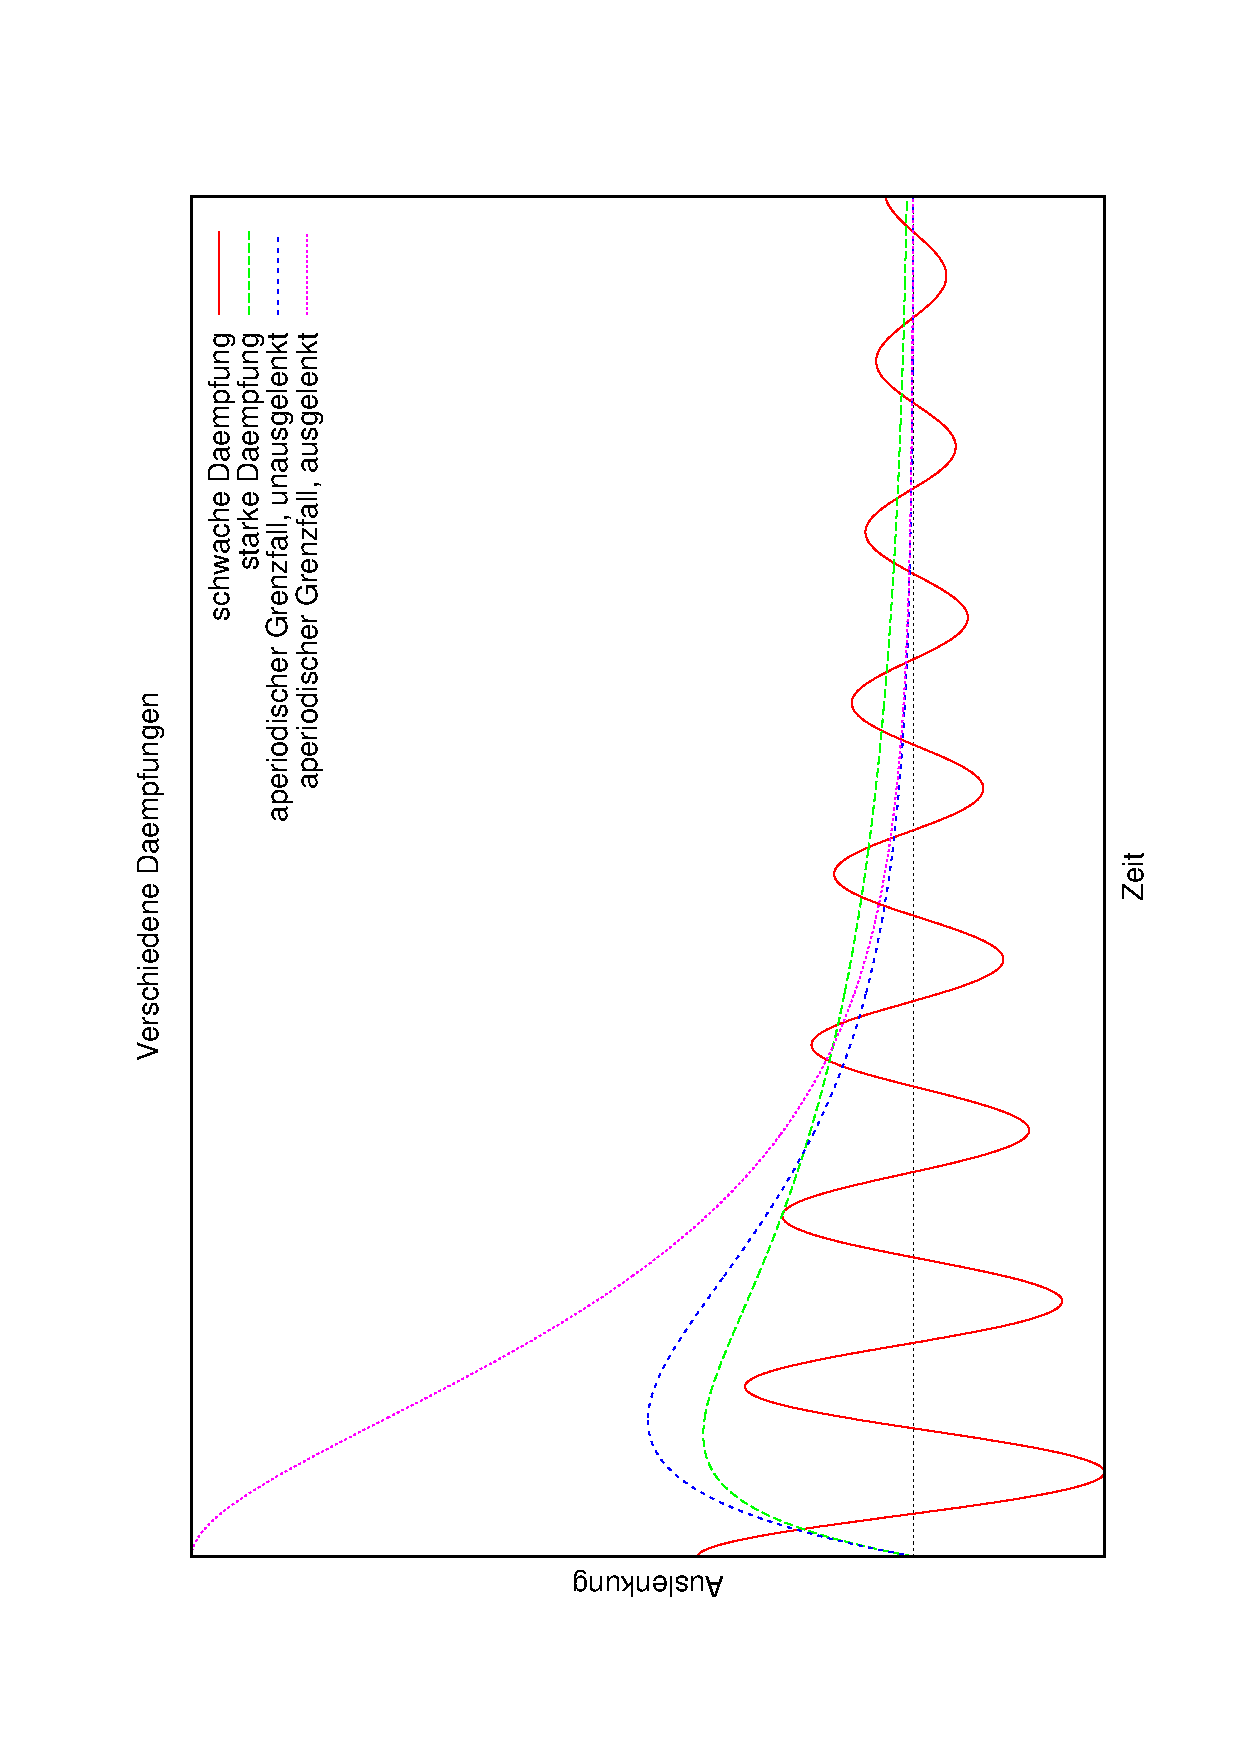
\includegraphics[width=0.7\textwidth,angle=-90]{bilder/dampf01}
   \caption[Dämpfungen einer Schwingung]{Verschiedene D"ampfungen
     einer Schwingung; die Amplituden und Frequenzen wurden
     willk"urlich gew"ahlt.}
   \label{abb_daempf}
\end{figure}









\section{St"orung}
\label{kap_storung}





Nun wollen wir noch eine \textbf{externe Kraft} angreifen lassen:
\begin{equation}
   \label{eq:107}
   F_{ext} = \hat F_{ext} \cos (\omega_{ext} t)
\end{equation}
D.h. unser Pendel wird die ganze Zeit "uber von au"sen periodisch
angeregt. Dem Pendel bleibt nach einer "`Einschwingphase"' nichts
anderes "ubrig, als mit der Frequenz $\omega_{ext}$ zu schwingen. 

Weil periodisch Energie zugef"uhrt wird, wird die D"ampfung praktisch
mit ausgeglichen.

In der \textbf{Bewegungsgleichung} steuert $F_{ext}$ jetzt auch einen Teil
zu $F_T$ bei und wir erhalten analog:
\begin{equation}
   \label{eqn_gestoerte-schwingung}
\boxed{   m\ddot x + \gamma \dot x + Dx = F_{ext} }
\end{equation}




\subsection{\emph{Then-A-Wonder-Occurs}-Ansatz}
\label{kap_then-a-wonder-occurs-ansatz}


Unser neuer \textbf{Ansatz} lautet:
\begin{equation}
   \label{eq:117}
   x(t) = \hat x \sin(\omega_{ext} t + \varphi_{ext})
\end{equation}
Dabei ist $\varphi_{ext}$ die \emph{Phasendifferenz} zuwischen Erreger
und Oszillator (Pendel).

Durch Ableiten und Einsetzen\footnote{Then a wonder occurs} erh"alt man
\begin{eqnarray}
   \label{eq:118}
   \varphi_{ext} &=& \arctan \frac{- \omega_{ext}}{\frac{m}{\gamma}
     (\omega_0^2 - \omega_{ext}^2)}\\
\hat x &=& \frac{\hat F}{\sqrt{(\omega_0^2 - \omega_{ext}^2)^2m^2 +
    {\omega_{ext}^2 \gamma^2}}}
\end{eqnarray}
Siehe dazu Abb. \ref{abb_ampl-erzw}.





\subsection{Allgemeiner Ansatz}
\label{kap_allgemeiner-ansatz-1}


Wir f"uhren $K = \frac{\hat F_{ext}}{m}$ ein, um die DGL
\eqref{eqn_gestoerte-schwingung} umzuformulieren (Achtung: Hier ist
$\delta$ nicht mehr wie oben gew"ahlt!):
\begin{equation}
   \label{eq:125}
   \ddot x + 2 \delta \dot x + \omega_0^2x = K \cos \omega t
\end{equation}
Dann erhalten wir auf der linken Seite die linke Seite von
Gl. \eqref{eqn_schwingung-reibung}. D.h. wir haben hier mit
\eqref{eq:125} eine inhomogene DGL, die wir l"osen, indem wir zu einer
homogenen L"osung (wie \eqref{eq:124} -- oder besser gleich \eqref{eqn_schwache-daempfung}) eine
\emph{\index{Partikul"arl"osung}Partikul"arl"osung} addieren. Diese
Partikul"arl"osung ist nach dem \emph{Ansatz vom Typ der Rechten Seite}
einfach 
\begin{equation}
   \label{eq:129}
   x_p(t) = \hat x_p \cos (\omega_p t + \varphi_p)
\end{equation}
wobei $\omega_p = \omega_{ext} = \omega$ die Erregerfrequenz ist.

D.h. wir erhalten insgesamt als L"osung
\begin{equation}
   \label{eqn_erregt}
\boxed{   x(t) = \hat x_h \exp(-\delta t) \cdot \cos(\omega_h t + \varphi_h)
   + \hat x_p \cdot \cos (\omega_p t + \varphi_p) }
\end{equation}
Wobei  $\omega_h$ die Frequenz der entsprechenden ged"ampften,
\emph{nicht angeregten} Schwingung --
s. Kap. \ref{kap_allgemeiner-ansatz} -- ist.

Wir wollen nun einige \textbf{qualitative Untersuchungen} durchf"uhren:
Da im ersten Term eine exponentiell abnehmende Funktion steckt,
k"onnen wir den ersten Term f"ur gro"se $t$ ignorieren, da $\exp(-t)
\to 0$ f"ur $t \to \infty$ und die Cosinus-Terme beschr"ankt sind.

Nehmen wir an, diese "`\index{Einschwingphase}Einschwingphase"' ist vorbei, dann haben wir
als L"osung nur noch den zweiten Term aus \eqref{eqn_erregt} -- also im
Prinzip \eqref{eq:129}.

Setzen wir diese L"osung in \eqref{eq:125} ein, erhalten wir f"ur $t =
\frac{\pi}{2 \omega_p}$
\begin{equation}
   \label{eq:132}
   \left ( \omega_p^2 - \omega_0^2 \right ) \sin \varphi_p - 2 \delta
   \omega_p \cos \varphi_p = 0
\end{equation}
und damit
\begin{equation}
   \label{eq:134}
 \tan \varphi_p =      \frac{ 2 \delta
   \omega_p}{  \omega_p^2 - \omega_0^2 }
\end{equation}
Und f"ur $t = 0$ gilt:
\begin{equation}
   \label{eq:133}
  \hat x_p \cdot  (\omega_p^2 - \omega_0^2) \cos \varphi_p + 2 \delta
  \hat x_p \omega_p \sin\varphi_p = -K
\end{equation}
Und damit
\begin{eqnarray}
   \label{eq:135}
   \hat x_p \cos \varphi_p &=& \frac{-K - 2 \delta
  \hat x_p \omega_p \sin\varphi_p}{\omega_p^2 - \omega_0^2} \\
\label{eq:136}
\hat x_p \sin \varphi_p &=& \frac{-K - \hat x_p \cdot \left ( \omega_p^2 -
   \omega_0^2 \right ) \cos \varphi_p }{2 \delta \omega_p}
\end{eqnarray}
Da $(\hat x \cos \phi)^2 + (\hat x \sin \phi)^2 = {\hat x}^2$ ist,
k"onnen wir Gl.~\eqref{eq:135} und \eqref{eq:136}  quadrieren und
addieren und erhalten unter Verwendung von \eqref{eq:132}: 
\begin{equation}
   \label{eq:137}
   \hat x_p = \frac{K}{\sqrt{(\omega_0^2 - \omega_p^2)^2 + (2\delta\omega_p)^2}}
\end{equation}













\subsection{F"alle}
\label{kap_falle}



Wir unterscheiden drei verschiedene F"alle f"ur die anregende Frequenz:
\begin{description}[\setlabelstyle{\bfseries\slshape}]
\item[Kleine Frequenzen $\omega_{ext} \ll \omega_0$]
Der Oszillator folgt dem Erreger unmittelbar.

Oszillator und Erreger schwingen in Phase: $\varphi_{ext} =0$ Die
Amplitude f"ur kleine $\omega_{ext}$ ist 
$$
\hat x = \frac{\hat F}{m\omega_0^2} ~\Leftrightarrow ~ \hat F = D \cdot
\hat x
$$

\item["Ahnliche Frequenzen $\omega_{ext} \approx \omega_0$] 
Die Amplitude erreicht ihren H"ochstwert f"ur $\omega_{ext} \equiv
\omega_0$; die Phasenverschiebung geht dann unabh"angig von der
D"ampfung gegen $\varphi_{ext} \to 90^\circ$.

Hier tritt auch die \textbf{\index{Resonanzkatastrophe}Resonanzkatastrophe} ein: Wenn die
D"ampfung $\gamma$ klein genug ist, geht $\hat x \to \infty$.

\item[Hohe Frequenzen $\omega_{ext} \gg \omega_0$] 
Die Amplitude verschwindet.

Der Oszillator kann der Erregung nicht mehr folgen; $\varphi \to 180^\circ$.
\end{description}


\begin{figure}
   \centering
\subfigure[Amplitude im Abh"angigkeit von Anregungsfrequenz]{  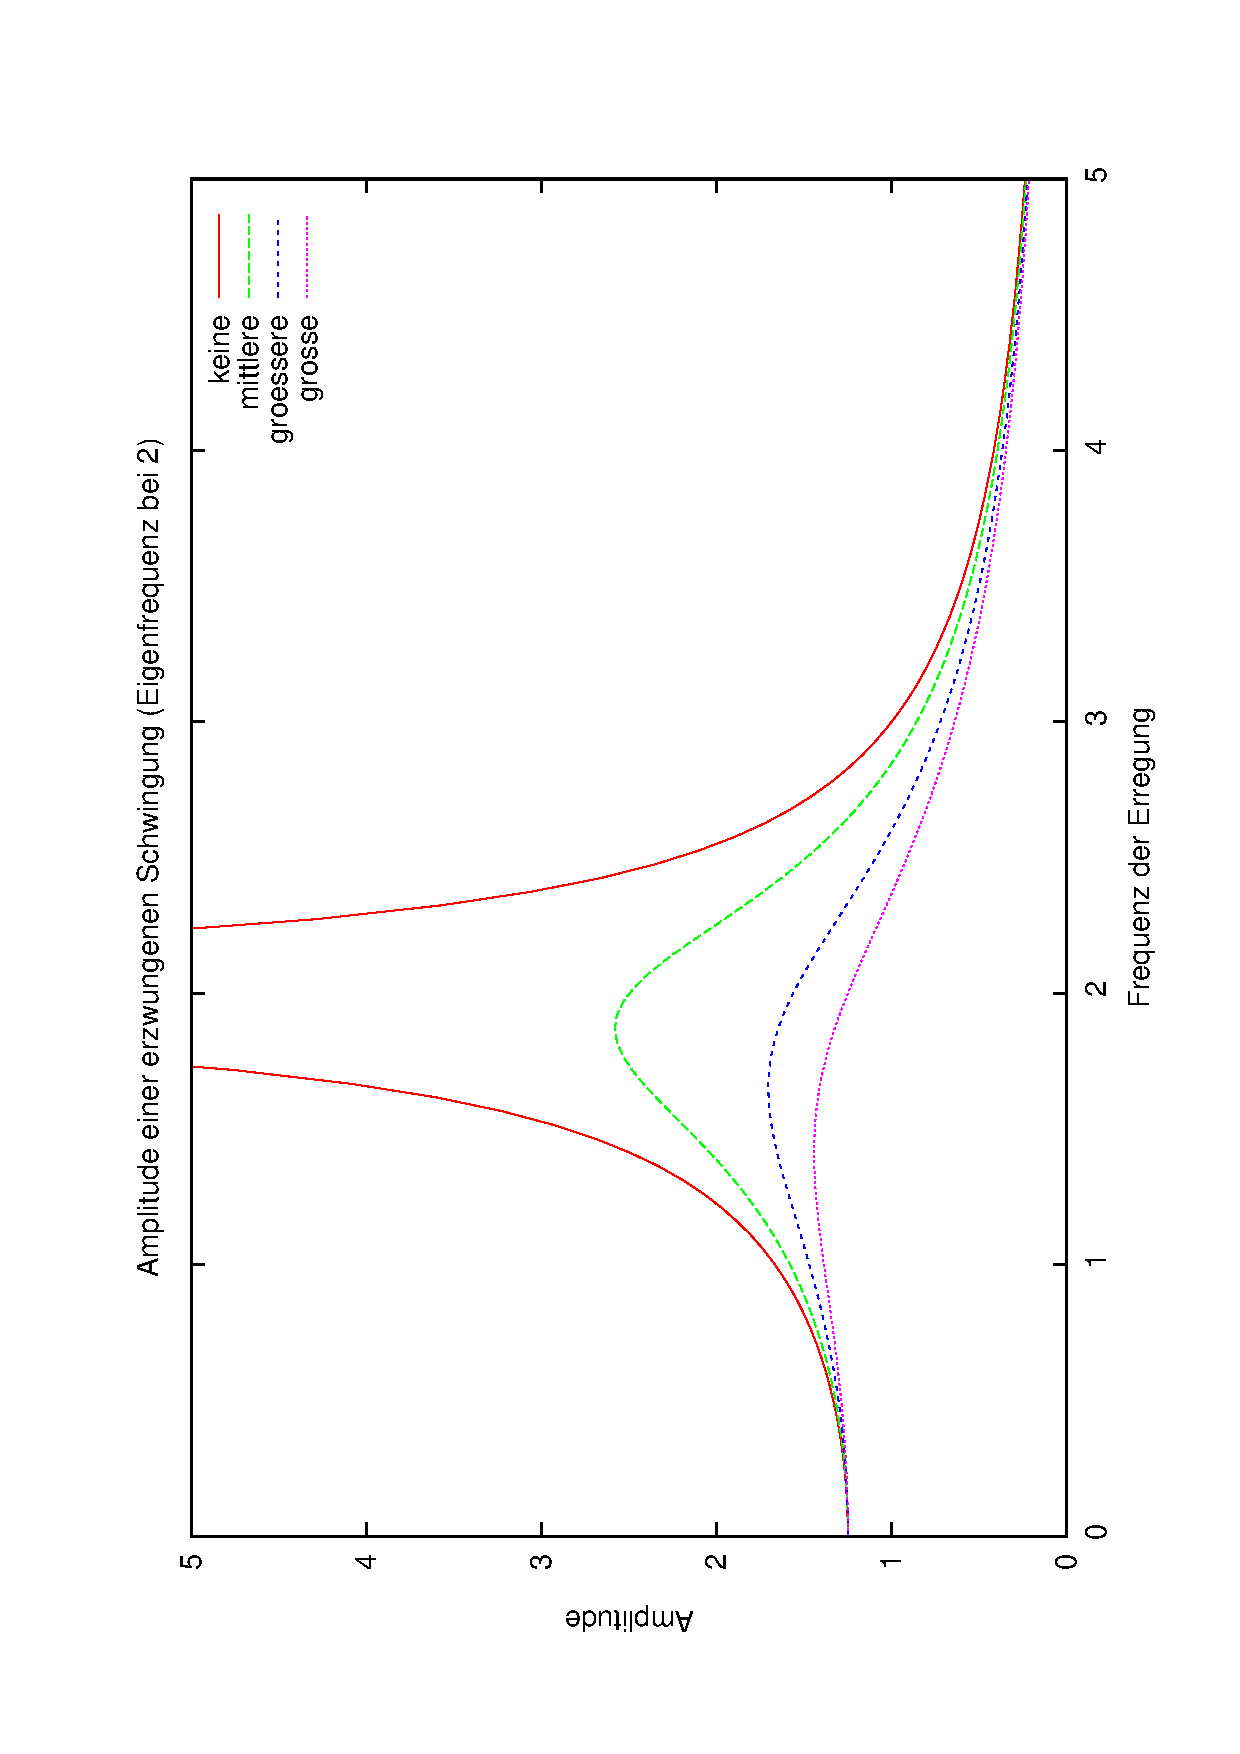
\includegraphics[width=0.8\textwidth,angle=-90]{bilder/ampl-erzw01}} 
\subfigure[Phase in Abh"angigkeit von Anregungsfrequenz]{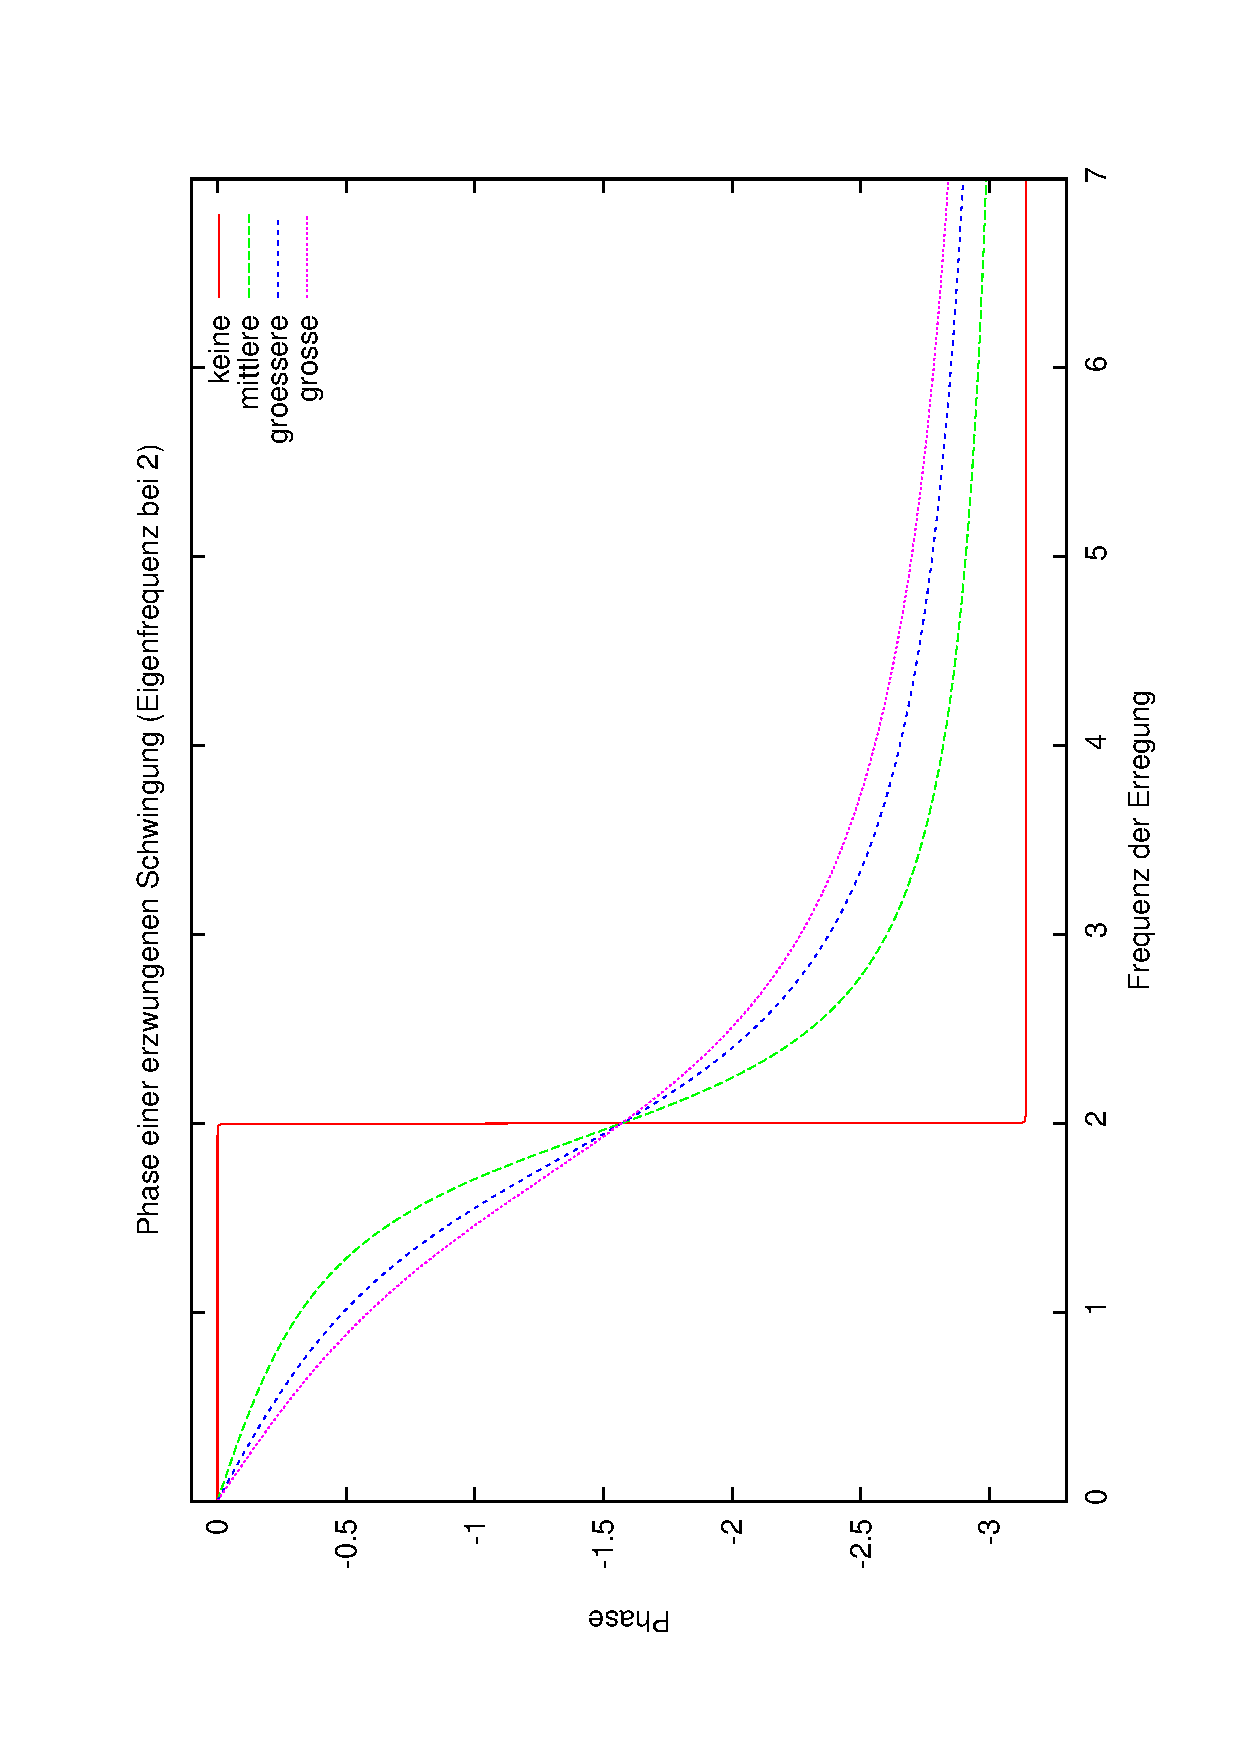
\includegraphics[width=0.8\textwidth,angle=-90]{bilder/phase-erzw01}}
\caption[Amplituden und phasen einer erzwungenen Schwingung]{Amplitude
  und Phase einer Erzwungenen Schwingung bei verschiedenen D"ampfungen
  -- siehe Gl. \eqref{eq:117} \eqref{eq:118}}
   \label{abb_ampl-erzw}
\end{figure}







   





\section{Gekoppelte Schwingungen}
\label{kap_gekoppelte-schwingungen}

Wir lassen zwei Pendel nebeneinander pendeln und verbinden ihre
Gewichte durch eine Feder. Dadurch haben wir zwei (harmonische oder
ged"ampfte) Schwingungen, die von der jeweils anderen Schwingung
angeregt werden. 

Wir f"uhren zwei getrennte Koordinatensysteme ein; das eine Pendel
beschreiben wir mit $x$, das andere mit $y$. Nun "uben die Pendel keine
Kr"afte aufeinander aus, wenn sie gleichphasig (syncron) schwingen;
dann ist der Abstand zwischen ihnen konstant und die Feder wird weder
gedehnt noch gestaucht. Nur wenn die Feder ihre L"ange ver"andert, "ubt
sie eine Kraft auf die beiden Schwinger aus. Die Kraft, die der
\emph{linke} Schwinger erf"ahrt ist\footnote{Lassen wir $x$ konstant
  und vergr"o"sern $y$ so wirkt wirklich eine Federkraft l"angs der
  $x$-Achse auf den linken Schwinger.}
\begin{equation}
   \label{eq:138}
   F_{ext,\text{links}} = D \cdot(y-x)
\end{equation}

D.h. wir k"onnen die Differenzialgleichung der nicht ged"ampften,
angeregten Schwingung aufstellen:
\begin{equation}
   \label{eq:139}
   m \ddot x + Kx = F_{ext} = D(y-x) ~\Leftrightarrow ~ \ddot x +
   \underbrace{\frac{K}{m}}_{\omega_0^2}x + \frac{D}{m}(x-y) = 0
\end{equation}
Dabei verwenden wir $K$ als Konstante f"ur die \emph{R"uckstellkraft}
und $\omega_0$ die Eigenfrequenz des linken Pendels ohne Koppelung.

F"ur den rechten Schwinger gilt entsprechend:
\begin{equation}
   \label{eq:140}
   \ddot y + \omega_0^2 y + \frac{D}{m} (y-x) = 0
\end{equation}


\subsection{Entkoppeln mit Ansatz}
\label{kap_entkoppeln-mit-ansatz}


Als Ans"atze w"ahlen wir hier zwei harmonische Schwingungen:
\begin{equation}
   \label{eq:141}
   x = \hat x \cdot \sin (\omega t + \varphi) ~\text{ und } ~
   y = \hat y \cdot \sin (\omega t + \varphi)
\end{equation}
Einsetzen ergibt wieder:
\begin{eqnarray}
   \label{eq:142}
   -\omega^2 x + \omega_0^2 x + \frac{D}{m} x &=& \frac{D}{m}y\\
   -\omega^2 y + \omega_0^2 y + \frac{D}{m} y &=& \frac{D}{m}x
\end{eqnarray}
 Multipliziert man die
Gleichungen erh"alt man 
\begin{equation}
   \label{eq:143}
  \left  (-\omega^2 + \omega_0^2 + \frac{D}{m} \right ) ^2 = \left ( \frac{D}{m}
   \right )^2
\end{equation}
Dabei muss man beachten, dass wenn man die Gl. \eqref{eq:142}
miteinander multipliziert, in jedem Summanden $x\cdot y$ steckt und so
darf man durch dieses teilen. Wir teilen also praktisch bevor wir die
Gleichungen multiplizieren schon durch $x\cdot y$ -- weil wir wissen, dass
diese Terme sowieso herausfallen. Deshalb kann man diese Rechnung sehr
einfach machen. 

Es gilt weiter:
\begin{equation}
   \label{eq:144}
   -\omega^2 + \omega_0^2 + \frac{D}{m} = \pm \frac{D}{m}
\end{equation}
Und wir haben also zwei Ergebnisse:
\begin{enumerate}[F{a}ll I]
\item $\omega = \omega_0$ wenn wir das "`$+$"' von "`$\pm$"' w"ahlen:
$$
x = y
$$
(erhalten wir, wenn wir $\omega = \omega_0$ in \eqref{eq:141} links
einsetzen).

Die Pendel schwingen \index{gleichphasig}in Phase
("`\emph{gleichphasig}"') und so wird die Feder weder gedehnt noch
gestaucht.
\item $\omega = \sqrt{ \omega_0^2 + 2\frac{D}{m} }$ wenn wir das
   "`$-$"' von "`$\pm$"' w"ahlen:
$$
x = -y
$$
Die Pendel schwingen \emph{\index{gegenphasig}gegenphasig} d.h. sie
erreichen gleichzeitig ihre maximale Auslenkung ung gleichzeitig ihre
minimale Auslenkung.
\end{enumerate}



\begin{figure}
   \centering
   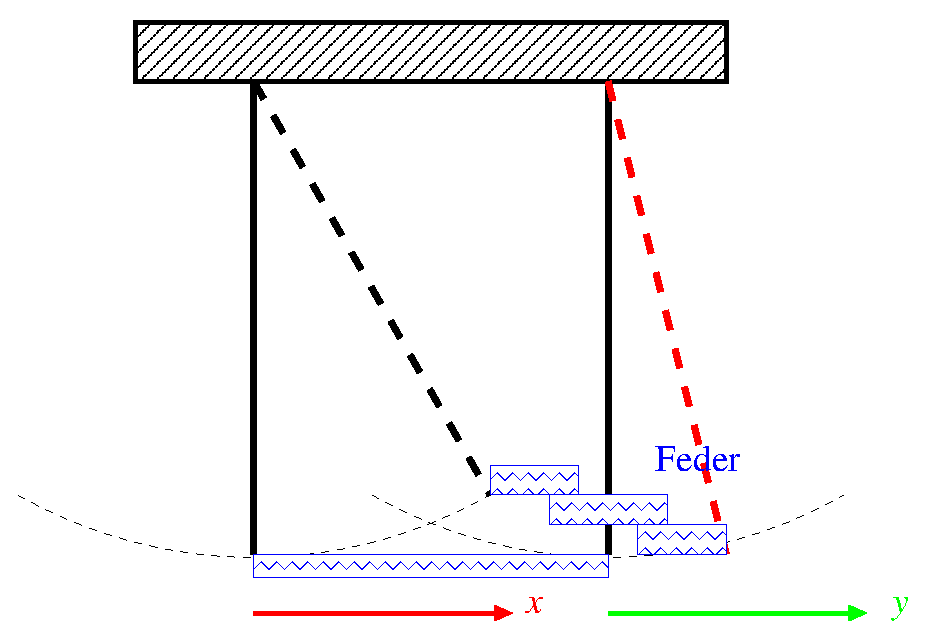
\includegraphics[width=0.5\textwidth]{bilder/gekoppelt}
   \caption[Gekoppeltes Fadenpendel]{Gekoppeltes Fadenpendel (Die
     gestauchte Feder soll die Verk"urzung der Feder als "Uberlappung
     symbolisieren)}
   \label{abb_gekoppelt}
\end{figure}

\begin{Wichtig}
   Aus diesen beiden Schwingungszust"anden kann man jede Bewegung
   gekoppelter Pendel durch "Uberlagerung erzeugen.
\end{Wichtig}
Bspw. ist in Abb. \ref{abb_schwebung} die Schwingung der beiden Pendel
dargestelle, wenn nur eines der beiden zu Anfang der Schwingung
ausgelenkt war. Man nennt diese Verhalten
\textbf{\index{Schwebung}Schwebung}. Hier wechselt die kinetische
Energie st"andig zwischen den beiden Pendeln hin und her.

\begin{figure}
   \centering
   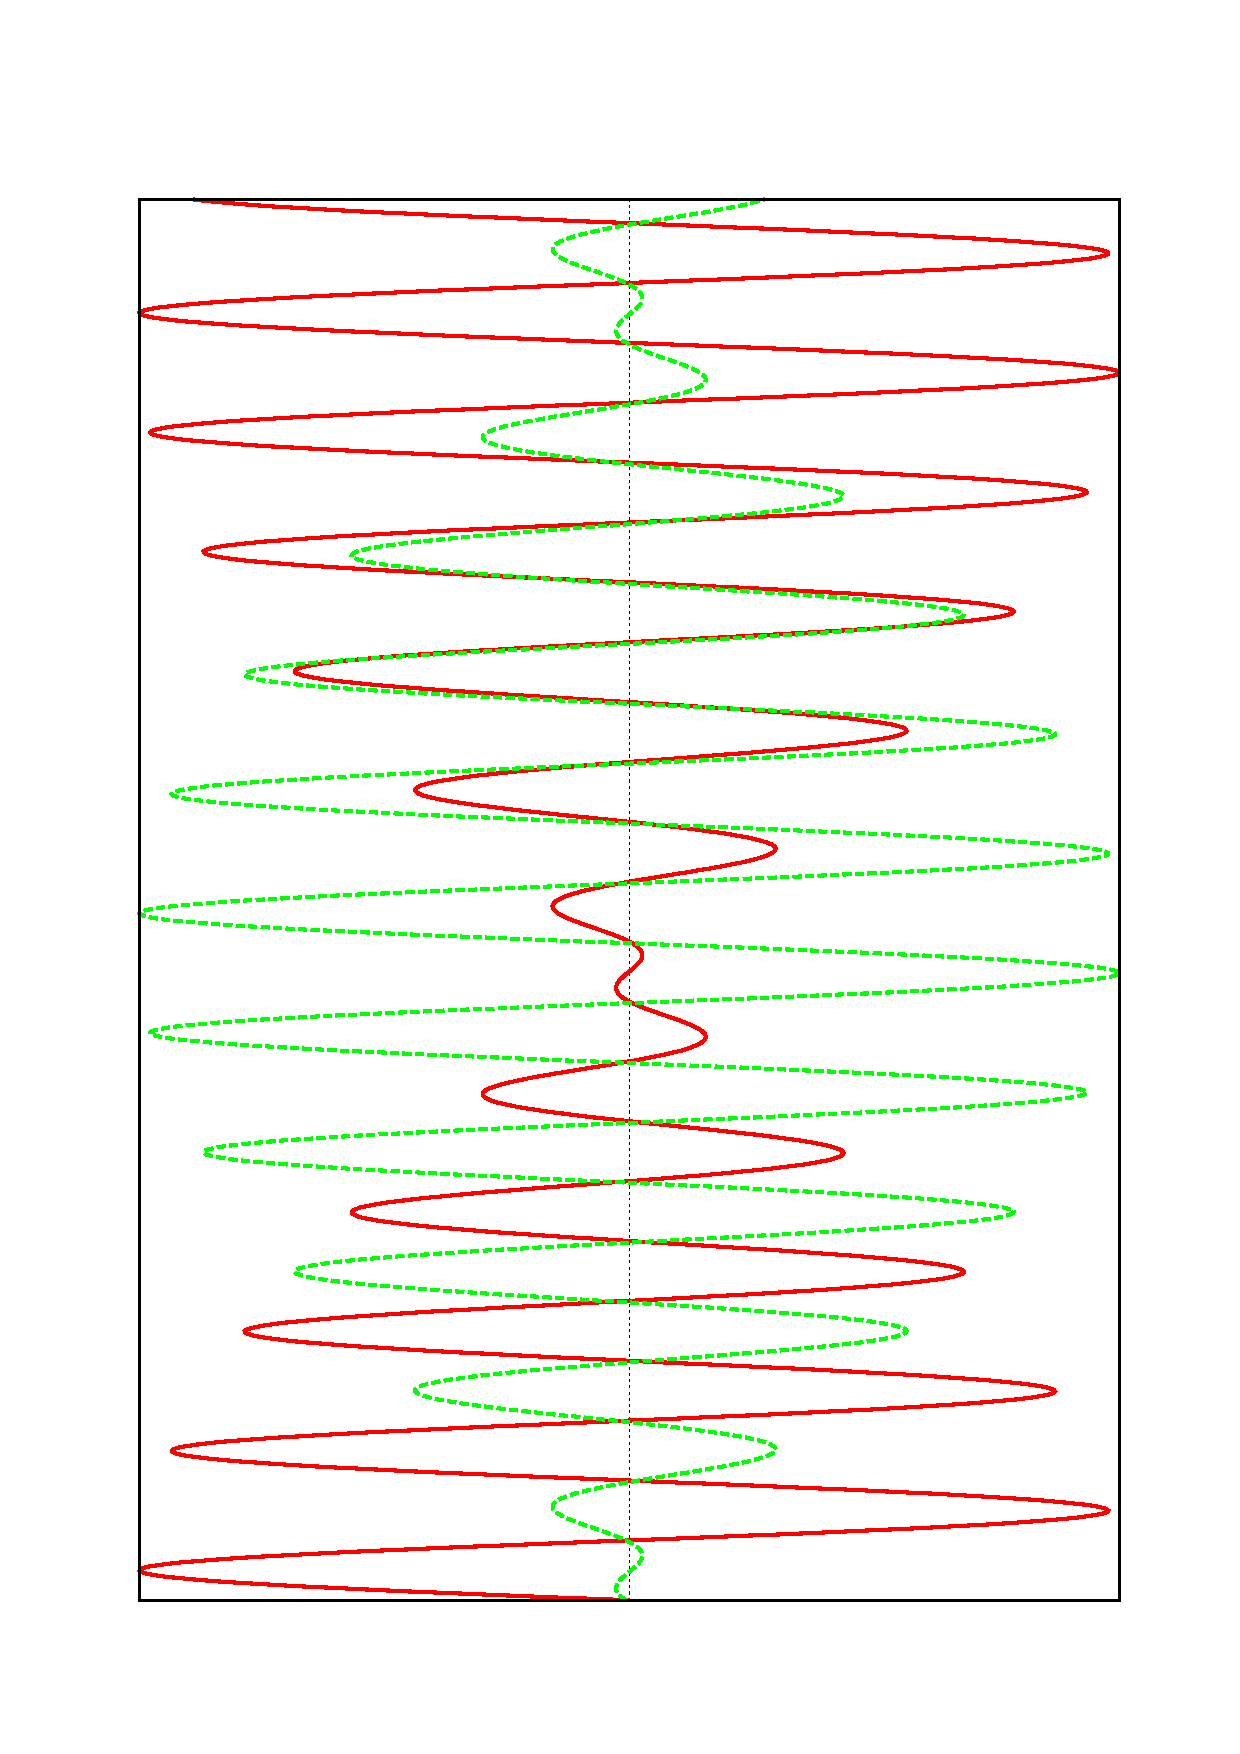
\includegraphics[width=0.7\textwidth,angle=-90]{bilder/schwebung}
   \caption[Schwebung]{Schwebung: Nur eines der beiden gekoppelten
     Pendel ist zu Anfang ausgelenkt}
   \label{abb_schwebung}
\end{figure}




\subsection{Entkoppeln ohne Ansatz}
\label{kap_entkoppeln-ohne-ansatz}

Oben haben wir den Sinusansatz wieder durch \emph{\index{Clever
    guess}Clever guess}
(vgl. Kap. \ref{kap_then-a-wonder-occurs-ansatz}) gefunden. Wir wollen
das Problem nochmal besprechen, wobei wir einen etwas allgemeineren
Ansatz w"ahlen. Wir gehen wieder aus von den Bewegungsgleichungen
\begin{equation}
   \label{eq:24}
   \begin{split}
      m \ddot x + Kx + D(x -y) = 0\\
      m \ddot y + Ky + D(y -x) = 0
   \end{split}
\end{equation}
aus, nur dass wir sie diesmal einmal addieren und einmal
subtrahieren:
\begin{equation}
   \label{eq:25}
   \begin{split}
      m (\ddot x - \ddot y) + K(x - y) + 2D(x - y) = 0 \\
      m (\ddot x + \ddot y) + K(x + y) = 0 
   \end{split}
\end{equation}
Durch "`\index{Koordinatentransformation"'}Koordinatentransformation"'
erh"alt man daraus die zwei neuen Bewegungsgleichungen
\begin{equation}
   \label{eq:26}
   \begin{split}
      m \ddot u + Ku + 2D u = 0 \text{ oder } m \ddot u + (K + 2D)u = 0\\
      m \ddot v + Kv = 0
   \end{split}
\end{equation}
Die wir einfach l"osen k"onnen: Es handelt sich um \emph{harmonische
  Schwingungen}, die wir aus Kap. \ref{kap_freie-schwingung}
kennen. So kennen wir auch die L"osung daf"ur:
\begin{equation}
   \label{eq:27}
   u(t) = \hat u \cdot \cos(\sqrt{\frac{K+2D}{m}} \cdot t + \varphi)
   \text{ und }
v(t) = \hat v \cdot \cos(\sqrt{\frac{K}{m}}\cdot t + \psi)
\end{equation}
Auf die eigentlichen Koordinaten $x$ und $y$ kommen wir nun wieder
durch Addition und Subtraktion von $u$ und $v$:
\begin{equation}
   \label{eq:28}
   x = \frac{1}{2}(v+u) \text{ und } y = \frac{1}{2}(v-u)
\end{equation}
"Uber die Anfangsbedingungen erh"alt man Gr"o"sen f"ur $\hat u$ und $\hat
v$ (und $\varphi$ und $\psi$), die dar"uber bestimmen, welchen Anteil
$u$ und $v$ an $x$ und $y$ haben.






\subsection{Entkoppeln mit Matrix}
\label{kap_entkoppeln-mit-matrix}

Wir stellen nun den Schwinger durch einen \emph{Vektor} dar: $\vec z =
(x,y)^T$. Damit ver"andert sich \eqref{eq:24} zur Vektorgleichung
\begin{equation}
   \label{eq:22}
   m \ddot{\vec z} + 
   \begin{pmatrix}
      K+D & -D\\
      -D & K+D
   \end{pmatrix} \cdot \vec z
= 
\vec 0 ~ \text{ oder } ~ 
   \begin{pmatrix}
      m \frac{\diff ^2}{\diff t^2} + K+D & -D\\
      -D & m \frac{\diff ^2}{\diff t^2} + K+D
   \end{pmatrix} \cdot \vec z = \vec 0
\end{equation}
Als allgemeinen Ansatz machen wir
(vgl. Kap. \ref{kap_allgemeiner-ansatz})
\begin{equation}
   \label{eq:23}
   \vec z = \vec z(t) = \vec Z \cdot \E^{\lambda t}
\end{equation}
Damit erh"alt man
\begin{equation}
   \label{eq:29}
     \begin{pmatrix}
      m \lambda^2 + K+D & -D\\
      -D & m \lambda^2 + K+D
   \end{pmatrix} \cdot \vec z = \vec 0 
~\text{ oder } ~ \Mat A \cdot \vec z = \vec 0
\end{equation}
Damit diese Gleichung nicht trivial wird (also $\vec z = \vec 0$),
muss $\det \Mat A \equiv 0$ werden\footnote{Sonst (also $\det \Mat A
  \neq 0$) sind die Spalten von $\Mat A$ linear unabh"angig und damit
  k"onnen sie nur durch die triviale Linearkombination zu $0$ addiert
  werden.}. F"ur die $2\times 2$-Matrix ist dies noch machbar: 
\begin{equation}
   \label{eq:200}
   \left (m \lambda^2 + K+D \right)^2 - D^2 \equiv 0
\end{equation}
und so erh"alt man f"ur $\lambda$ die Identit"aten:
\begin{equation}
   \label{eq:201}
   \lambda = -\sqrt{-\frac{K}{m}} \text{, } 
\lambda = \sqrt{-\frac{K}{m}}
\text{, }
\lambda =-\sqrt{-\frac{K}{m}-\frac{2\,D}{m}}
\text{, }
\lambda=\sqrt{-\frac{K}{m}-\frac{2\,D}{m}}
\end{equation}
Dabei haben wir stets negative Wurzeln -- also Komplexe Zahlen! Dies
wiederum bedeutet, dass in unserem Ansatz \eqref{eq:23} der $\E$-Term
eine Schwingung beschreibt. Die Korrekte L"osung besteht aus einer
Linearkombination von vier Termen nach \eqref{eq:23} wobei alle $\vec
Z$ -- theoretisch -- frei bestimmbar sind. Weil wir jedoch wieder nur
an \emph{rellen} L"osungen interessiert sind, m"ussen die $\vec Z$
jeweils f"ur die beiden ersten und die beiden Letzten $\lambda$ aus
\eqref{eq:201} voneinander das komplexe Konjugat sein; damit bekommen
wir aber weiterhin \emph{vier} Freiheitsgrade. Wie in
Kap. \ref{kap_allgemeiner-ansatz} bekommen wir zwei (komplexe)
Vektoren $\vec Z$ und zwei \emph{Phasenverschiebungen} der Cosini.

Hier haben wir die ganze Zeit "uber angenommen, dass die beiden Massen
$m$ gleich sind, ebenso wie dass die beiden Federn $K$ gleich hart
sind. Wenn dem \emph{nicht} so w"are, w"are die L"osung mit diesem Ansatz
ebenso zu bestimmen -- nur ein wenig komplizierter. Die Ausdr"ucke (f"ur
\emph{ein} $\lambda$) sind so lange, dass sie nicht in eine Zeile hier
passen...
















\section{"Uberlagerung von Schwingungen -- Interferenz}
\label{kap_uberlagerung-con-schwingungen-interferenz}

\subsection{Gleiche Frequenz}
\label{kap_gleiche-frequenz}

\begin{eqnarray}
\nonumber
   x &=& A \sin (\omega t)\\
\nonumber
   y &=& B \sin (\omega t)\\
   \label{eq:145}
   x+y &=& (A+B) \cdot \sin (\omega t)
\end{eqnarray}

\subsection{Unterschiedliche Frequenz}
\label{kap_unterschiedliche-frequenz}

\begin{eqnarray}
\nonumber
   x &=& A \sin(\omega_1 t)\\
\nonumber
   y &=& A \sin(\omega_2 t)\\
   \label{eq:146}
   x+y &=& 2A \cdot \sin\left ( \frac{\omega_1 + \omega_2}{2} \cdot t \right
   ) \cdot \cos \left ( \frac{\omega_1 - \omega_2}{2}\cdot t \right )
\end{eqnarray}
Wir benutzen dabei ein Additionstheorem f"ur $\sin(\vartheta) +
\sin(\vartheta)$.  Siehe auch
Kap. \ref{kap_phasen-und-gruppengeschwindigkeit-bei-uberlagerung}.



\subsection{Beliebige Schwingungen}
\label{kap_beliebige-schwingungen}

Dank der \textsc{Fourier}-Analyse ist es m"oglich, jede periodische
Funktion aus Sinus- und Cosinus-Schwingungen zusammenzusetzen.

In der Realit"at ist das nicht immer m"oglich, weil bspw. die Federh"arte
nicht konstant ist und so die formal mit Sinusschwingungen gel"osten
Bewegungen eigentlich gar keine solche absolvieren.









\section{Fortschreitende Welle}
\label{kap_fortschreitende-welle}


\begin{Wichtig}
   [\index{Energietransport}\index{Massentransport}Energietransport]
   Bei einer Schwingung wird \emph{Energie} transportiert. Die
   Massenteilchen selbst bleiben am Ort und schwingen nur um eine
   Ruhelage.
\end{Wichtig}


\subsection{Wellengleichung und Definitionen}
\label{kap_wellengleichung-und-definitionen}



Wir gehen von der Schwingung in der Zeit an einem Ort (wir denken sie
uns im Ursprung) mit der Gleichung 
\begin{equation}
   \label{eq:147}
   y_0(t) = \hat y \sin(\omega t + \varphi_0)
\end{equation}
"uber zu einer Schwingung, die zus"atzlich noch eine r"aumliche
Komponente hat.
\begin{Def}
   [\index{Wellenl"ange}Wellenl"ange $\lambda$]
Der r"aumliche Abstand zwischen zwei phasengleich schwingenden Punkten
einer Welle.
\end{Def}
% Die R"aumliche Komponente:

% \begin{equation}
%    \label{eq:148}
%    y(x)
% = \hat y \sin \left (\frac{-2\pi}{\lambda}x \right ) = 
% -\hat y \sin \left (2\pi\frac{x}{\lambda} \right )
% \end{equation}


Die "Uberlegung ist, dass je weiter in $x$-Richtung wir uns von dem in
\eqref{eq:147} betrachteten Schwinger wegbewegen, die Schwingung in
einer anderen Phase ist. Wenn man ein ganzzahliges Vielfaches der
Wellenl"ange zur"uckgelegt hat, soll die Phase wieder die gleiche
sein. Deshalb teilen wir die Entfernung $x$ durch die Wellenl"ange
$\lambda$ und haben so die Entfernung normiert als \emph{Anzahl von
  Wellenl"angen}. Genau so oft hat die Welle bis zum Punkt $x$ schon
eine komplette Periode hinter sich. Eine Periode des Sinus ist $2\pi$
lang -- also hat die Welle bis zum Punkt $x$ die Phasendifferenz
$2\pi\frac{x}{\lambda}$ zum Ursprungspunkt der mit Gl.  \eqref{eq:147}
beschrieben wird. Also hat der Punkt $x$ die Phase
$$
\varphi(x) =
\varphi_0 + 2\pi\frac{x}{\lambda}
$$


Um die Schwingung im Punkt $x$ zur Zeit $t$ zu berechnen, k"onnen wir
die Schwingung im Punkt $x = 0$ betrachten -- also Gl. \eqref{eq:147}
verwenden. % Im Punkt $x$ hat die Schwingung aber eine andere Phase --
% und zwar muss man von der Phase $\omega t + \varphi_0$ die
% Phasendifferenz $2\pi\frac{x}{\lambda}$ abziehen, weil der
% Schwingungszustand, der aktuell in $x = 0$ herrscht, noch
% $2\pi\frac{x}{\lambda}$ \emph{vor} dem aktuellen Zustand liegt.
Indem wir von der Phase der Schwingung im Punkt $x$ den Wert
$\varphi(x)$ abziehen, erhalten wir die Phase, die der Punkt in $x=0$
zur Zeit $t$ hat und k"onnen so $y(x,t)$ ausrechnen.

Es ergibt sich die Wellengleichung
\begin{equation*}
y = y(x,t) = \hat y \cdot \sin \left ( \omega \cdot t - \frac{2\pi}{\lambda}
   \cdot x \right ) 
\end{equation*}
Eine Kleine Erinnerung: Wir k"onnen die Gleichung auch schreiben als
\begin{equation*}
   y = y(x,t) = \hat y \cdot \sin \left ( \frac{2\pi}{T} \cdot t - \frac{2\pi}{\lambda}
   \cdot x \right )
\end{equation*}
Damit sieht man den Zusammenhang von Periodendauer $T$ und Wellenl"ange
$\lambda$ noch besser. Wie man die Frequenz $\omega$ als Abk"urzung
$\omega = \frac{2\pi}{T}$ verwendet, verwendet man als Abk"urzung von $\frac{2\pi}{\lambda}$:
\begin{Def}
   [(\index{Kreiswellenzahl}Kreis)\index{Wellenzahl}\index{Wellenvektor}Wellenzahl
   $k$] mit 
   \begin{equation}
      \label{eq:205}
      k = \frac{2\pi}{\lambda}
   \end{equation}
\end{Def}
Damit k"onnen wir die Gleichung f"ur $y(x,t)$ noch weiter umschreiben:
\begin{equation}
   \label{eqn_welle_1dim}
   \boxed{
y = y(x,t) = \hat y \cdot \sin \left ( \omega \, t - k \, x \right ) }
\end{equation}

\bigskip


\begin{Def}
   [\index{Ausbreitungsgeschwindigkeit}Ausbreitungs- /
   \index{Phasengeschwindigkeit}Phasengeschwindigkeit $c$ oder
   $c_\text{Phase}$] Ein bestimmter Schwingungszustand der Schwingung
   -- also eine gewisse Phase -- bewegt sich mit der Geschwindigkeit
   $c$ fort.
   \begin{equation}
      \label{eqn_def_ausbreitungsgeschw}
      c_\text{Phase} = \frac{\lambda}{T} = \frac{\omega}{2\pi} \lambda = \lambda
      \cdot \nu
=
\frac{\omega}{k}
   \end{equation}
\end{Def}
mit der Kreiswellenzahl $k$ (s. \eqref{eq:205}) und
\begin{Def}
   [\index{Periodendauer}Periodendauer $T$]
An einem Ort dauert es $T$ bis sich der selbe Schwingungszustand
wieder eingestellt hat.
\end{Def}
D.h. die Gleichung 
$$
c = \frac{\lambda}{T}
$$
entspricht 
$$
v = \frac{s}{t}
$$




\subsection{Differenzielle Form der Wellengleichung}
\label{kap_differenzielle-form-wellengleichung}

Im Speziellen Fall f"ur nur eine Dimension gilt:
\begin{equation}
   \label{eq:149}
   \frac{\partial^2}{\partial t^2} y = c^2 \cdot
   \frac{\partial^2}{\partial x^2} y
\end{equation}
Der Allgemeine Fall ber"ucksichtigt noch mehr Raumdimensionen $x_i$:
\begin{equation}
   \label{eq:150}
   \frac{1}{c^2} \frac{\partial^2 }{\partial t^2} \vec y - \sum_{i=1}^n
   \left ( \frac{\partial ^2}{\partial x_i^2} \vec y \right ) = 0
\end{equation}
Dabei k"onnen wir dies mit dem \textsc{Laplace}-Operator $\Delta$
umschreiben zu:
\begin{equation}
   \label{eqn_wellengleichung}
\boxed{
  \frac{1}{c^2} \frac{\partial^2 }{\partial t^2} \vec y - \Delta
  \vec y = 0 
}
\end{equation}

Wenn wir nun unsere Gleichung \eqref{eqn_welle_1dim} einsetzen,
so erhalten wir:
\begin{equation}
   \label{eq:151}
   \frac{\omega^2}{c^2} = \frac{4\pi^2}{\lambda^2}
\end{equation}
und damit wieder den Zusammenhang aus
\eqref{eqn_def_ausbreitungsgeschw}. Die von uns anschaulich
hergeleitete L"osung stimmt also.









\section{Arten von Wellen}
\label{kap_arten-von-wellen-1}

Wir unterscheiden zwei Typen:
\begin{description}[\setlabelstyle{\bfseries\slshape}]
\item[\index{Transversalwellen}Transversalwellen]  Schwingen \emph{senkrecht} zu ihrer
   Ausbreitungsgeschwindigkeit (bspw. Wasserwellen)
\item[\index{Longitudialwellen}Longitudialwellen] Schwingen \emph{parallel} zur
   Ausbreitungsrichtung (bspw. Schallwellen\footnote{Der Mensch kann
     Schallwellen mit Frequenzen von $\nu \in [20\operatorname{Hz};
     20\, 000 \operatorname{Hz}]$ wahrnehmen.})
\end{description}




\section{Interferenz}
\label{kap_interferenz}



Zwei Wellen durchdringen sich im Allgemeinen ohne Probleme -- also
gehen \emph{unver"andert} weiter. In dem Bereich, in dem sie sich
durchdringen \textbf{"uberlagern} sie sich; ihre Auslenkungen addieren
sich.

Im besonderen Fall hat man zwei Wellen der selben Frequenz $\nu$; hier
ergeben sich zwei Spezialf"alle:
\begin{Def}[konstruktive und destruktive Interferenz]
   Bei \textbf{\index{konstruktive Interferenz}konstruktiver
     Interferenz} hat die Summe der Wellen eine maximale Amplitude
   ($|\hat y_1| +| \hat y_2|$), bei \textbf{\index{destruktive
       Interferenz}destruktiver Interferenz} wird die Amplitude der
   "Uberlagerung minimal ($||\hat y_1| - |\hat y_2||$).
\end{Def}
Haben die Wellen sogar die gleiche Amplitude $\hat y$, so hat die
"Uberlagerung bei konstruktiver Interferenz die Amplitude $2 \hat y$
und bei destruktiver Interferenz verschwindet die Amplitude der
"Uberlagerung.

Wir definieren
\begin{Def}
   [\index{Gangunterschied}Gangunterschied $\Delta s$]
Der k"urzeste r"aumliche Abstand zwischen zwei gleichen
Schwingungszust"anden zwischen zwei verschiedenen ("uberlagernden) Wellen.
\end{Def}
und analog dazu
\begin{Def}
   [\index{Phasendifferenz}Phasendifferenz $\Delta \varphi$]
Der Unterschied der Phasen zweier Wellen am selben Ort.
\end{Def}
Es gilt der Zusammenhang
\begin{equation}
   \label{eq:152}
   \Delta \varphi = \frac{2\pi}{\lambda} \cdot \Delta s \text{ ~ oder
   } \frac{\Delta \varphi}{\Delta s} = k
\end{equation}
wobei $k$ die \emph{Kreiswellenzahl} aus \eqref{eq:205} ist.

Wir betrachten gleichf"ormige (also gleiche Frequenz
bzw. Wellenl"ange und Amplitude) Wellen $x$, $y$ und $z$:
\begin{equation*}
   x = A \cos(\omega t - kx) \text{, } y = A \cos(\omega t  - k
   (x+\Delta s))
\text{ und } z = A \cos(\omega t - kx + \Delta \varphi)
\end{equation*}
Anschaulich ist klar, dass sich genau dann eine maximale Amplitude von
$2A$ ergibt, wenn die Argumente der Cosini sich um vielfache von
$2\pi$ unterscheiden und genau dann die minimale Amplitude von $A-A =
0$, wenn sich die Argumente um $\pi, 3\pi, 5\pi,...$
unterscheiden. F"ur die \emph{Phasendifferenz} $\Delta \varphi$ kann man so
sofort die gew"unschten Bedingungen finden (s. \eqref{eq:202} und
\eqref{eq:203}). F"ur den \emph{Gangunterschied} dagegen vergleichen
wir $x$ mit $y$ und sehen, dass $k \Delta s$ f"ur konstruktive
Differenz vielfache von $2\pi$ sein m"ussen und f"ur destruktive
Interferenz $\pi, 3\pi, 5\pi,...$. Dies h"atte man auch aus
Gl. \eqref{eq:152} schlie"sen k"onnen. Es folgen damit die Bedingungen:

\begin{Wichtig}
   [Bedingung: \index{Konstruktive Inverferenz}Konstruktive
   \index{Interferenz!Konstruktive}Interferenz] liegt vor, wenn
\begin{eqnarray}
   \label{eq:155}
   \Delta s &=& \lambda \cdot n ~ ~ ~ n \in \mathbb Z\\
\label{eq:202}
   \Delta\varphi &=& 2\pi \cdot n~ ~ ~ n \in \mathbb Z
\end{eqnarray}
\end{Wichtig}

und

\begin{Wichtig}
   [Bedingung: \index{Destruktive Interferenz}Destruktive
   \index{Interferenz!Destruktive}Interferenz] liegt vor, wenn
\begin{eqnarray}
\label{eq:157}
   \Delta s &=& n \cdot \lambda + \frac{\lambda }{2} ~ ~ ~ n \in
   \mathbb Z\\
\label{eq:203}
   \Delta\varphi &=& n \cdot 2\pi  + \pi~ ~ ~ n \in \mathbb Z
\end{eqnarray}
\end{Wichtig}




\section{Phasen- und Gruppengeschwindigkeit bei "Uberlagerung}
\label{kap_phasen-und-gruppengeschwindigkeit-bei-uberlagerung}

Wir wollen zwei Wellen mit verschiedenen Wellenl"angen und Frequenzen
"uberlagern. Mit der Kreiswellenzahl $K_i = \frac{2\pi}{\lambda_i}$ 
gilt
\begin{eqnarray}
   \label{eq:164}
   u = A \sin (\omega_1 t - K_1 x)\\
   v = A \sin(\omega_2 t - K_2 x)
\end{eqnarray}
und mit  dem
Additionstheorem
$$
\sin \alpha + \sin \beta = 2 \sin \frac{\alpha + \beta}{2} \cos
\frac{\alpha - \beta}{2}
$$
weiter:
\begin{equation}
   \label{eq:165}
\boxed{ u + v = 
 2 A \cdot \sin \left ( \underbrace{\frac{\omega_1 + \omega_2}{2}}_\omega t - \underbrace{ \frac{K_1 +
     K_2}{2}}_K x \right ) \cdot \cos \left ( \frac{\omega_1 -
     \omega_2}{2}t - \frac{K_1  - K_2}{2}x \right )
}
\end{equation}
und damit
\begin{equation}
   \label{eq:166}
   u+v = 2A \cdot \sin (\omega t - K x) \cdot \cos \left ( \frac{1}{2} (\Delta \omega \cdot t -
   \Delta K \cdot x ) \right )
\end{equation}

Dabei ist der Cosinus-Term die \textbf{\index{Einh"ullende}Einh"ullende} der Schwingung,
weil die Maxima der Schwingung auf ihr liegen. Vgl. dazu
Abb. \ref{abb_einhuell}.

Nun wollen wir die Geschwindigkeit bestimmen, mit der sich die
Einh"ullende fortbewegt. Dazu betrachten wir ein Maximum der
Einh"ullenden; dazu muss $\cos = 1$ sein, also am besten:
\begin{equation}
   \label{eq:168}
   \left ( \frac{1}{2} (\Delta \omega \cdot t -
   \Delta K \cdot x ) \right ) = 0
\end{equation}
Wenn wir diese Gleichung mit $\frac{1}{2}$ k"urzen und nach
$\frac{x}{t} = v$ aufl"osen, bekommen wir genau
Gl. \eqref{eqn_gruppengeschwindigkeit}.\footnote{Dabei haben wir die
  Annahme gemacht, dass die Gruppengeschwindigkeit \emph{linear}, also
nicht beschleunigt ist. Diese Behauptund d"urfen wir machen, weil die
Wellen $u$ und $v$ selbst auch nicht beschleunigt waren, sondern sich
linear mit $c_\text{Phase}$ ausgebreitet haben.}


Wir definieren:
\begin{Def}[Gruppengeschwindigkeit $c_\text{Gruppe}$]
   Die Geschwindigkeit, mit der sich ein Schwingungszustand der
   Einh"ullenden bewegt ist die
   \textbf{\index{Gruppengeschwindigkeit}Gruppengeschwindigkeit}.
   \begin{equation}
      \label{eqn_gruppengeschwindigkeit}
      c_\text{Gruppe} = \frac{\Delta \omega}{\Delta K}
   \end{equation}
\end{Def}


\begin{figure}
   \centering
   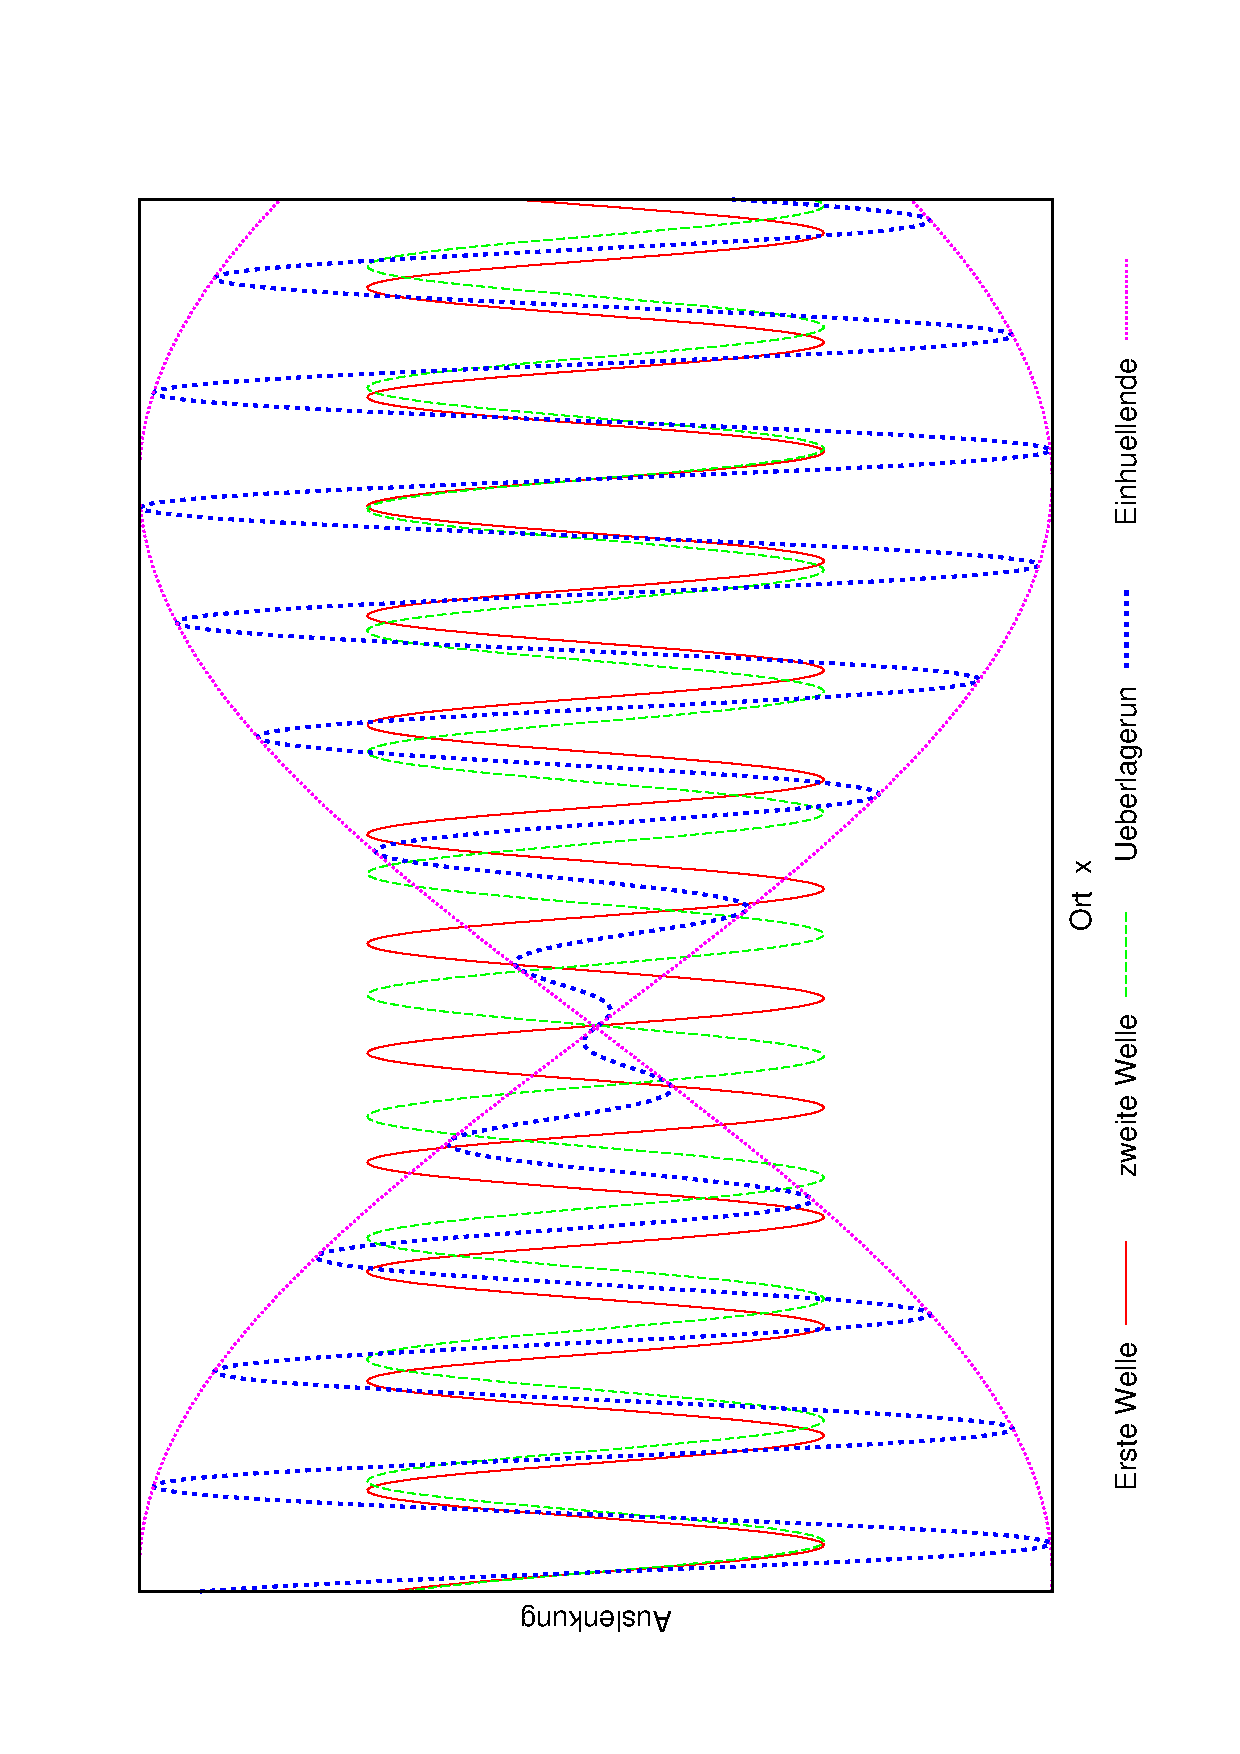
\includegraphics[width=0.7\textwidth,angle=-90]{bilder/einhuell}
   \caption[Überlappung zweier Wellen]{Zwei Wellen, deren
     "Uberlagerung und die Einh"ullende}
   \label{abb_einhuell}
\end{figure}

\bigskip
Als \textbf{Zusammenhang zwischen $c_\text{Gruppe}$ und
  $c_\text{Phase}$} finden wir, das bei einer infinitissimalen
Betrachtung von Gl. \eqref{eqn_gruppengeschwindigkeit}, wobei wir
$\omega$ durch $\omega = c_\text{Phase} \cdot K$ ersetzen:
\begin{equation}
   \label{eq:167}
   c_\text{Gruppe} = \frac{\diff \omega}{\diff K} = \frac{\diff
     (c_\text{Phase} \cdot K)}{\diff K} = c_\text{Phase}\frac{\diff K}{\diff K}
   + K \frac{\diff c_\text{Phase}}{\diff K}
\end{equation}
Wobei $\frac{\diff K}{\diff K} = 1$ ist. Wenn wir $K =
\frac{2\pi}{\lambda}$  einsetzen, erhalten wir so (weil $\diff K =
\diff \frac{2\pi}{\lambda} = - 2\pi \cdot \frac{1}{\lambda^2} \diff
\lambda$):
\begin{equation}
   \label{eq:169}
   c_\text{Gruppe} = c_\text{Phase} - K \frac{\lambda^2}{2\pi}
   \frac{\diff c_\text{Phase}}{\diff \lambda} 
=
\boxed{ c_\text{Phase} - \lambda \cdot \frac{\diff c_\text{Phase}}{\diff
  \lambda} = c_\text{Gruppe} }
\end{equation}




\section{Reflexion}
\label{kap_reflexion}

Wenn Wellen an einem \textbf{\index{festes Ende}festen Ende} auf ein
Hindernis treffen, so k"onnen die Enden des Wellentr"agers nicht
schwingen und damit keine Schwingungsenergie aufnehmen: Die Energie
der Welle wird wieder zur"uck auf die Welle geworfen.

Man kann sich vorstelle, dass die Welle die Wand mit Kraft $F$ bewegen
will (es aber nicht schafft) daf"ur die Wand die Welle aber mit der
Reactio $F$ in die Gegenrichtung zur"uckbewegt. 

Direkt an der Wand liegt ein \textbf{\index{Phasensprung}Phasensprung} von 
$$
\Delta \varphi = \pi
$$
vor, weil hier die Welle vom unteren Umkehrpunkt unvermittelt zum
bberen Umkehrpunkt "`springt"'.


\bigskip

Wenn der Wellentr"ager mit einem \textbf{\index{loses Ende}losen Ende} zuende geht, so
k"onnen die letzten Teilchen auf dem Wellentr"ager ungehindert
\emph{Schwingungen} ausf"uhren -- sie schwingen also "uber ihre Ruhelage
hinaus und wieder zur"uck und sorgen so daf"ur, dass wenn eine Welle mit
einer \textbf{\index{Schnelle}Schnelle}\footnote{die Bewegung der Schwingung
selbst --
also bei einer Transversalwelle die Geschwindigkeit, mit der ein
Massenteilchen sich senkrecht zur Ausbreitungsrichtung bewegt} nach
nach oben ankommt, nach der Reflexion wieder eine Schnelle nach oben
vorliegt. 

Hier liegt also kein Phasensprung vor:
\begin{equation}
   \label{eq:156}
   \Delta \varphi = 0
\end{equation}









\section{Stehende Wellen}
\label{kap_stehende-wellen}

\subsection{Entstehung und Aussehen}
\label{kap_entstehung-und-aussehen}



Wir betrachten zwei Wellen der gleichen Frequenz und Amplitude, die
aufeinander zulaufen. Ihre Wellengleichungen sind gegeben durch:
\begin{eqnarray*}
   u &=& A \sin \left (\omega t - \frac{2\pi}{\lambda}x \right )\\
   v &=& A \sin \left (\omega t + \frac{2\pi}{\lambda} x\right )
\end{eqnarray*}
Wenn wir diese Wellengleichungen addieren, um die "Uberlagerung zu
erhalten, k"onnen wir $A$ ausklammern und ein Additionstheorem des
Sinus anwenden und erhalten dann
\begin{equation}
   \label{eq:158}
   y = 2A \cos\left ( \frac{2\pi}{\lambda}x \right ) \cdot \sin \left
      ( \omega t \right )
\end{equation}
Wenn wir diese Welle zu verschiedenen Zeiten betrachten
(vgl. Abb. \ref{abb_stehend}), so f"allt auf, dass die $x$-Achse stets
an den selben Punkte geschnitten wird -- diese nennen wir
\textbf{Knoten} -- und dass es Stellen gibt, die sich maximal bewegen
-- \textbf{B"auche}. Wichtig ist dabei, dass weder Knoten noch B"auche
ihre $x$-Position ver"andern. Die Welle \emph{steht} also wirklich auf
einem Fleck und die einzelnen Massenpunkte f"uhren einfache harmonische
Schwingungen aus, wobei entscheidend ist \emph{wo} sie schwingen. Die
Teilchen, die direkt auf einem Knoten liegen, schwingen garnicht,
w"ahrend die Teilchen, die auf einem Bauch liegen, maximal schwingen.

Die Knoten treten in festen Abst"anden auf: An einem Ort ist der
Cosinusterm aus \eqref{eq:158} konstant. Wenn er also verschwindet,
verschwindet auch die Schwingung an dieser Stelle und wir haben einen
Knoten. Wenn der Cosinusterm dagegen maximal (also 1) wird, haben wir
einen Bauch. Die Knoten liegen also bei
\begin{equation}
   \label{eq:159}
x = \lambda \cdot \frac{2n+1}{4}
\end{equation}
mit $n \in \mathbb Z$ und die B"auche bei
\begin{equation}
   \label{eq:160}
   x = \lambda \cdot \frac{2n}{4}
\end{equation}
% F"ur die Amplitude $\hat y$ an einen Punkt, der von einem Bauch den
% Abstand $\delta$ hat, gilt, wenn $2A$ die maximale Amplitude der
% stehenden Welle ist (wenn $A$ die Amplitude einer einzelnen Welle
% war):
% \begin{equation}
%    \label{eq:161}
%    \hat y(\delta) = \pm 2A \cdot \sin \frac{4\delta}{\lambda}
% \end{equation}

\begin{figure}
   \centering
   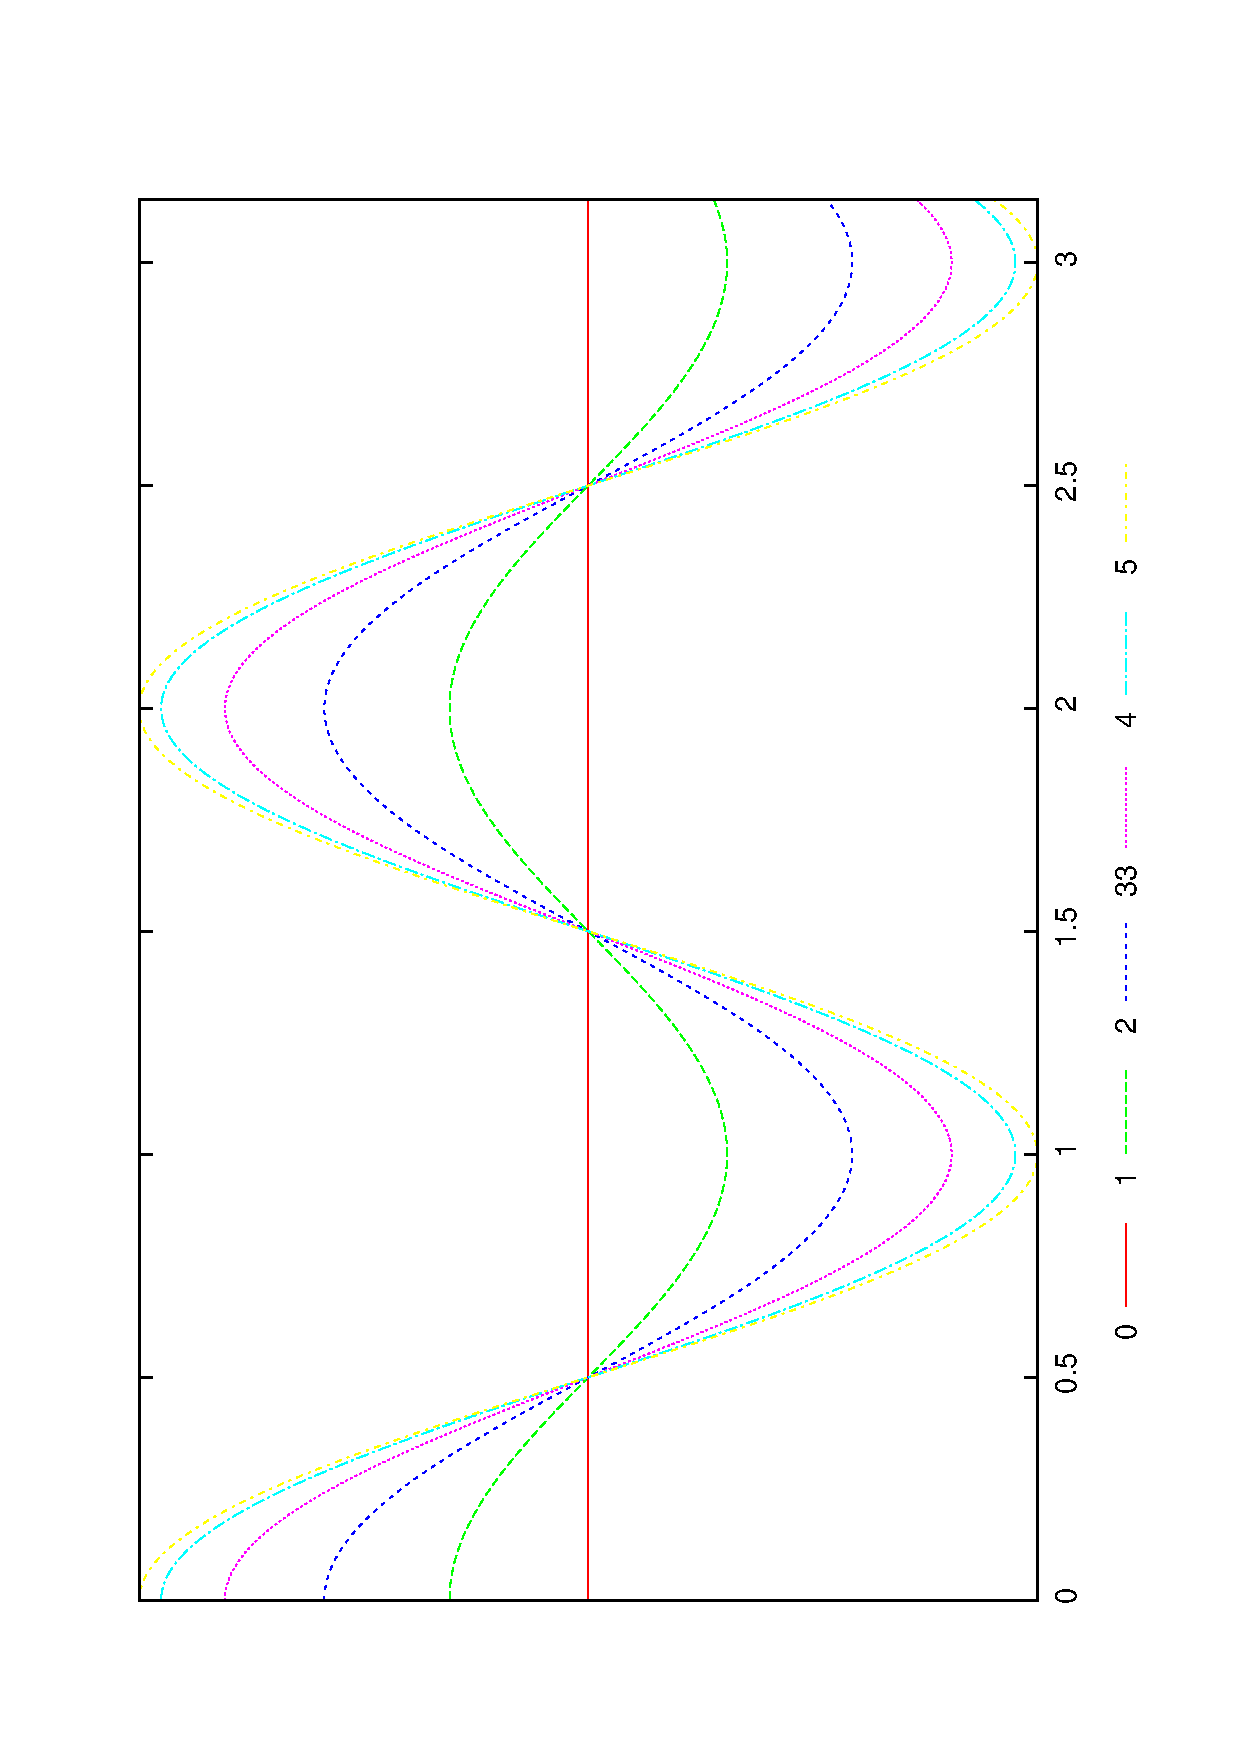
\includegraphics[width=0.7\textwidth,angle=-90]{bilder/stehend}
   \caption{Stehende Welle in 5+1 Zeitschritten}
   \label{abb_stehend}
\end{figure}




\subsection{Visualisierung}
\label{kap_visualisierung}


Wenn nun die schwingenden Teilchen so klein sind, dass wir sie nicht
mehr sehen k"onnen -- also wenn bspw. Luft als Longitudialwelle
schwingt -- dann m"ussen wir uns einen Trick einfallen lassen, um die
Schwingung trotzdem zu visualisieren.

Wenn Luftteilchen Schwingen, so bilden sich Knoten und B"auche der
Luftteilchen; diese werden als \emph{Geschwindigkeits}knoten und
-b"auche bezeichnet. Daneben gibt es noch \emph{Druck}b"auche und
-knoten. Dort wo ein Geschwindigkeitsknoten ist, sitzt ein Druckbauch,
einfach weil hier von links und von rechts st"andig Teilchen an das
ruhende Teilchen sto"sen und dr"ucken und so eine Kraft auf das Teilchen
aus"uben, die wir als Druck interpretieren.

Wir k"onnen nun die Bewegungsknoten visualisieren, indem wir bspw. in
einer R"ohre eine stehende Welle erzeugen, indem wir an beide Enden
Lautsprecher setzen, die den selben Ton spielen. Wenn wir nun kleine
Kr"umel -- bspw. B"arlappsporen, die besonders leicht und fein sind --
gleichm"a"síg im Rohr verteilen, so werden diese an den Stellen
"`weggewischt"', an denen die Geschwindigkeitsb"auche sind und in Ruhe
gelassen, wo die Geschwindigkeitsknoten liegen.  Wir bekommen also
kleine H"aufchen des Staubs bei den Geschwindigkeitsknoten.




\subsection{Auf beschr"anktem Wellentr"ager}
\label{kap_auf-beschranktem-wellentrager}

Nur die wenigsten Wellentr"ager die wir kennen sind unendlich
ausgedehnt. Die L"ange $L$ eines solchen Wellentr"agers bestimmt mit,
was f"ur stehende Wellen sich darauf bilden k"onnen.
\begin{Wichtig}
   Es bilden sich nur stehende Wellen bei characteristischen
   Frequenzen.
\end{Wichtig}
\begin{Def}[Eigenfrequenz $\omega_0$]
   Diese Frequenzen nennen wir
   \textbf{\index{Eigenfrequenz}Eigenfrequenz} des Wellentr"agers.
\end{Def}
Das liegt daran, dass die Enden des Wellentr"agers die Welle
reflektieren -- abh"angig davon, ob wir ein loses oder ein festes Ende
haben mit oder ohne Phasensprung
(s. Kap. \ref{kap_reflexion}). D.h. die Enden des Wellentr"agers sind
entweder selbst (Geschwindigkeits)B"auche (beim losen Ende) oder
(Geschwindigkeits)Knoten (bei festem Ende).

\begin{description}[\setlabelstyle{\bfseries\slshape}]
\item[Zwei feste Enden] Zwei Knoten haben stets den Abstand
   $\frac{\lambda}{2}$. Hat ein Wellentr"ager die L"ange $L$, so kann
   man genau $n$ B"auche darauf platzieren; damit die Knoten mit den
   R"andern zusammenfallen, muss $\frac{\lambda}{2}\, n = L$ sein oder:
%  Damit m"ussen den Abstand $L$ oder
%    $\frac{L}{2}$ oder $\frac{L}{n}$ haben ($n \in \mathbb N$) damit
%    Knoten und Enden des Wellentr"agers zusammenfallen. Da zwei Knoten
%    den Abstand $\frac{\lambda}{2}$ haben, gilt
   \begin{equation}
      \label{eq:153}
      \lambda_n^{(f,f)} = \frac{2\cdot L}{n} ~  ~ \text{ mit } n \in
      \mathbb N
   \end{equation}
Und mit der Ausbreitungsgeschwindigkeit $c$ und
\eqref{eqn_def_ausbreitungsgeschw} gilt f"ur die Frequenz:
\begin{equation}
   \label{eq:154}
   \nu_n^{(f,f)} = \frac{c}{2\cdot L} \cdot n
\end{equation}


\item[Ein festes und ein loses Ende] Zwei Knoten haben weiterhin den
   Abstand $\frac{\lambda}{2}$, aber diesmal kommt an einem Ende noch
   ein Abstand Knoten-Bauch, also $\frac{\lambda}{4}$, dazu.  Wir
   k"onnen auf dem Wellentr"ager also $n$ B"auche zwischen zwei Knoten
   und einen Bauch am losen Ende platzieren. Damit dies mit der L"ange
   "ubereinstimmt, muss $\frac{\lambda}{2}n + \frac{\lambda}{4} = L$
   gelten, oder\footnote{Das "`$-$"' im Nenner kommt daher, dass in
     dieser Gleichung $n\in \mathbb N$ sein soll! Damit man die
     l"angste Schwingung (also maximal gro"ses $\lambda$) damit
     darstellen kann, die einen Bauch und einen Knoten direkt an den
     Enden hat, braucht man im Nenner die $\frac{1}{2}$, und diese
     kann man nur erreichen, wenn man von $1$ die $\frac{1}{2}$
     \emph{abzieht}.}
   \begin{equation}
      \label{eq:162}
      \lambda_n^{(f,l)} = \frac{2 \cdot L}{n - \frac{1}{2}} ~  ~
      \text{ mit } n
      \in \mathbb N
   \end{equation}
und f"ur die Freqnenz:
\begin{equation}
   \label{eq:163}
   \nu_n^{(f,l)} = \frac{c}{2L} \cdot (n - \frac{1}{2} )
\end{equation}
\end{description}



\bigskip

\begin{Def}[Grund- und Oberschwingungen]
   Wir nennen die Schwingung mit der gr"o"st m"oglichen Wellenl"ange (also
   f"ur $n = 1$) \textbf{\index{Grundschwingung}Grundschwingung} und
   jede weitere Schwingung mit entsprechend k"urzerer Wellenl"ange
   $n$-te \textbf{\index{Oberschwingung}Oberschwingung}.
\end{Def}

Bei einem Musikinstrument haben die verschiedenen Oberschwingungen
verschiedene Amplituden. Das Verh"altnis dieser Amplituden zueinander
bestimmt die \textbf{\index{Klangfarbe}Klangfarbe} des Instruments.






\subsection{Funktionsprinzip von Fl"oten}
\label{kap_funktionsprinzip-von-floten}


Durch Lufteinblasen wird ein Blatt (eine Schneide) in Schwingungen
versetzt. Sie regt die Lufts"aule "uber sich in der Fl"ote zu
Schwingungen an (vgl. Abb. \ref{abb_floete}). Je n"aher die Luft am
Blatt ist, desto weniger Bewegungsfreiheit hat sie und schwingt hier
deshalb nur wenig, daf"ur aber entfernt vom Blatt st"arker.  In der N"ahe
des Blattes ist also der Druck gro"s, die Teilchenbewegung klein,
weiter entfernt anders herum.

Die schwingende Lufts"aule kann nun am Ende der Pfeife die Luft der
Umgebung zu Schwingungen anregen -- der Ton wird
"ubertragen. Gleichzeitig wird aber die Schwingung innerhalb der
Pfeife reflektiert und es bildet sich eine stehende Welle aus, wodurch
der Ton sich verst"arken kann (Durch \emph{\index{Resonanz}Resonanz}
kann sich die Amplitude "`aufschaukeln"').  Die \emph{H"ohe} des Tones
h"angt davon ab, wie gut das Blatt schwingen kann buzw. wie
gleichm"a"sig es angeregt wird und von der L"ange der Pfeife.

Wir unterscheiden zwischen \textbf{\index{gedeckte Pfeife}gedeckten}
Pfeifen, die ein Offenes und ein geschlossenes Ende haben und
\textbf{\index{offene Pfeife}offenen} Pfeifen, bei denen beide Enden
offen sind.

In einer Pfeife k"onnen verschiedene Frequenzen stehende Wellen
erzeugen, so lange die Bedingungen aus
Kap. \ref{kap_auf-beschranktem-wellentrager} eingehalten
werden. Vgl. dazu Abb. \ref{abb_pfeifen_schwingung}.


\begin{figure}
   \centering
   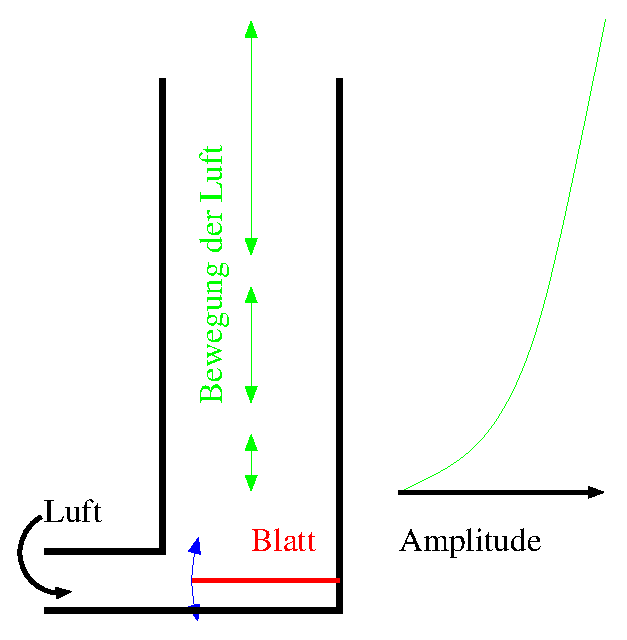
\includegraphics[width=0.5\textwidth]{bilder/floete}
   \caption{Prinzip einer Fl"ote}
   \label{abb_floete}
\end{figure}

\begin{figure}
   \centering
   \subfigure[Gedeckte Pfeife: Links geschlossenes, rechts offenes Ende]{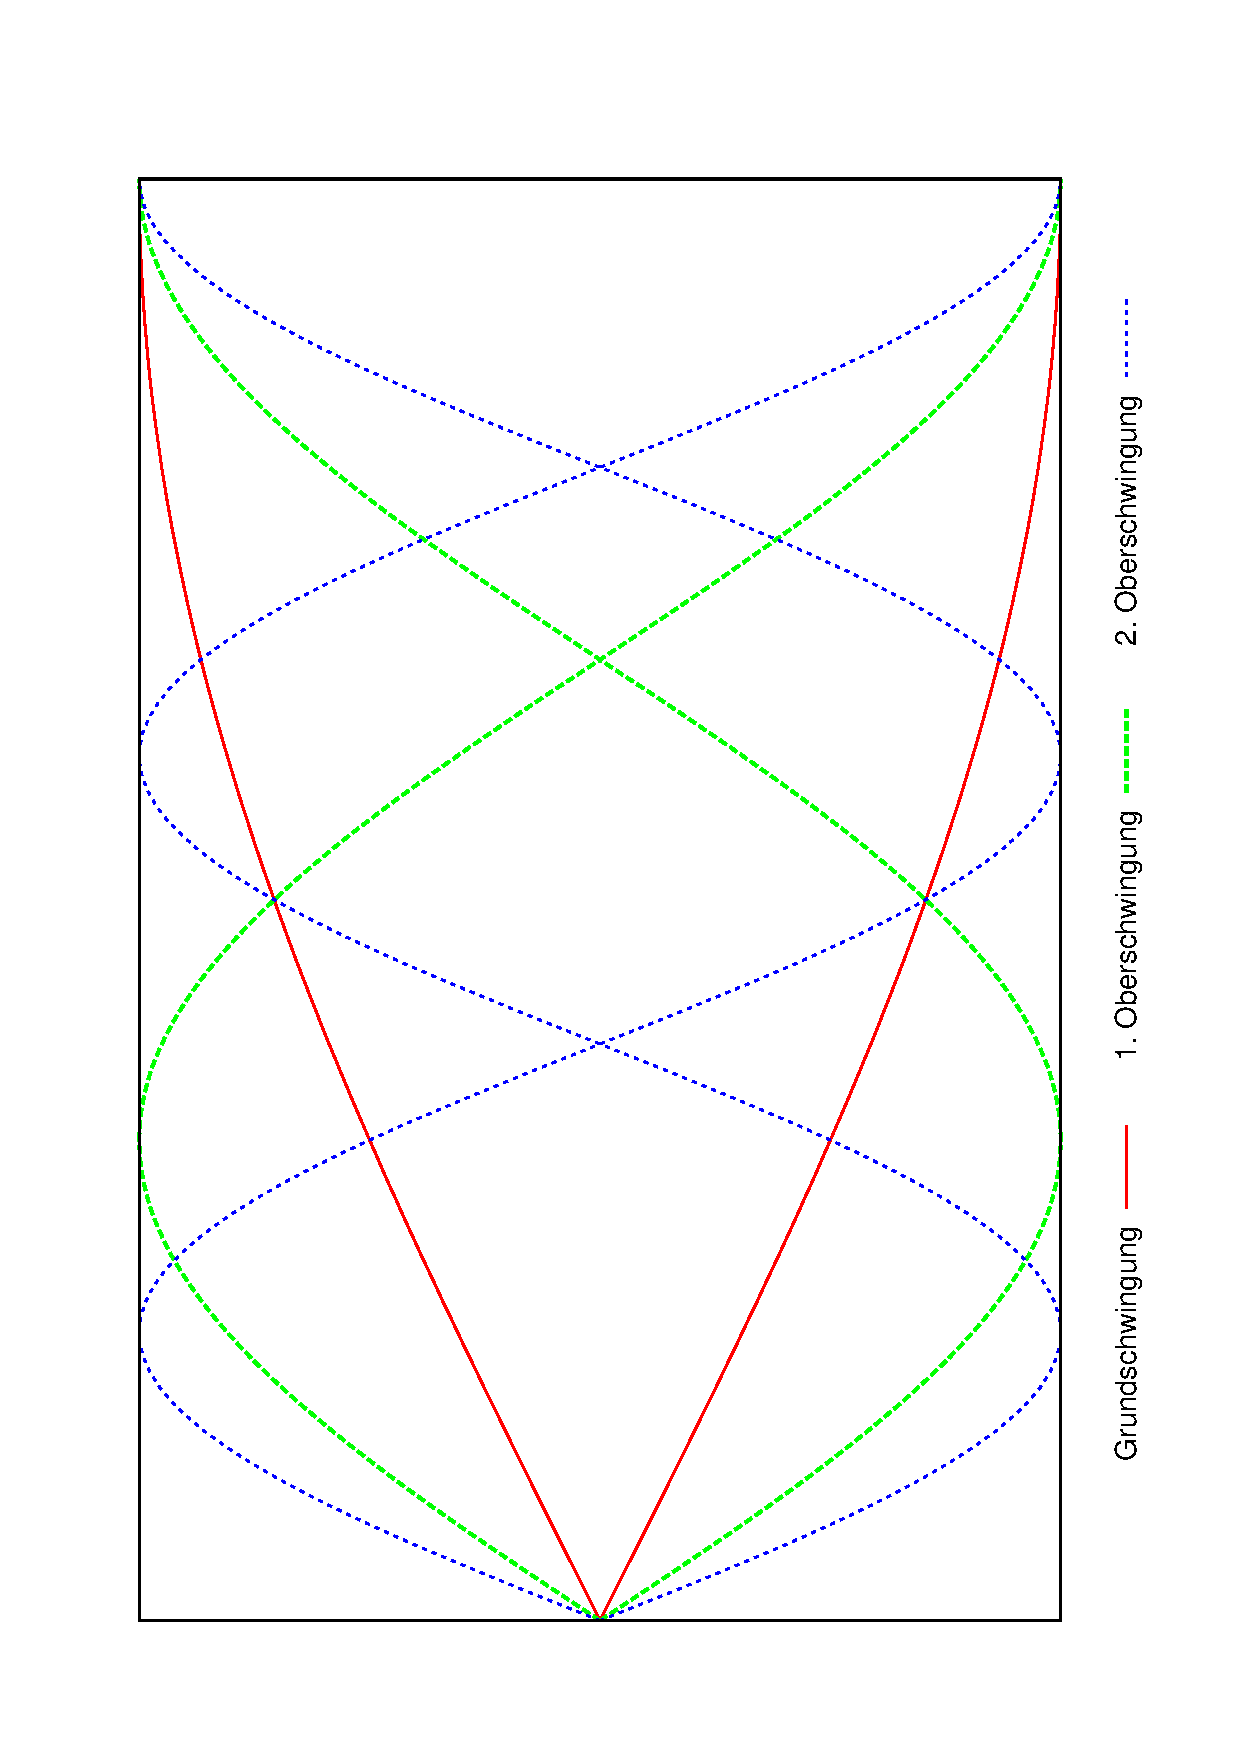
\includegraphics[width=0.3\textwidth,angle=-90]{bilder/gedeckt}}
   \subfigure[Offene Pfeife: Beide Enden offen]{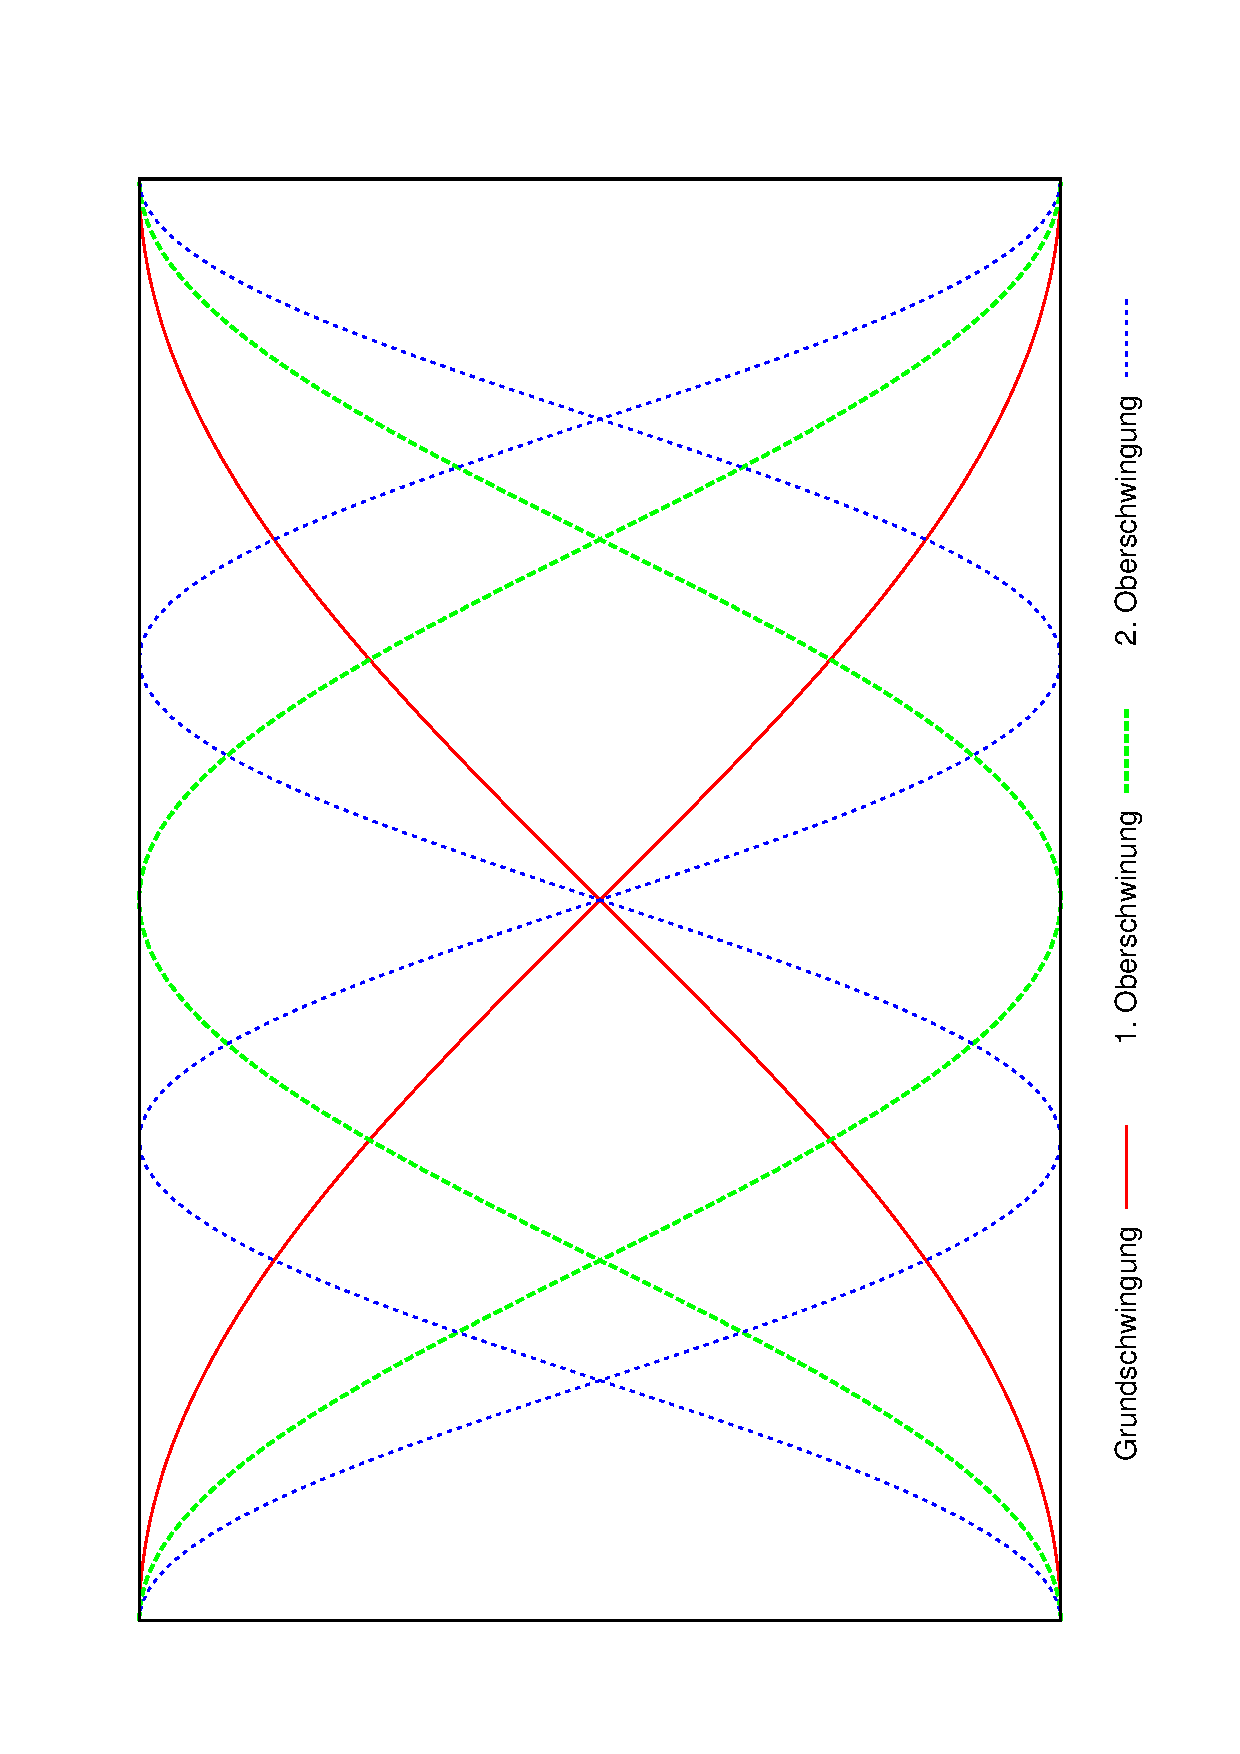
\includegraphics[width=0.3\textwidth,angle=-90]{bilder/offen}}
   \caption{Gedeckte und offene Pfeifen}
   \label{abb_pfeifen_schwingung}
\end{figure}









































%%%%%%%%%%%%%%%%%%%%%%%%%%%%%%%%%%%%%%%%%%%%%%%%%%%%%%%%%%%%%%%%%%

%%%%%%%%%%%%%%%%%%%%%%%%%%%%%%%%%%%%%%%%%%%%%%%%%%%%%%%%%%%%%%%%%

%%%%%%%%%%%%%%%%%%%%%%%%%%%%%%%%%%%%%%%%%%%%%%%%%%%%%%%%%%%%%%%%%


